%%%%%%%%%%%%%%%%%%%%%%%%%%%%%%%%%%%%%%%%%%
%                                        %
% Szablon pracy dyplomowej inzynierskiej %
%                                        %
%%%%%%%%%%%%%%%%%%%%%%%%%%%%%%%%%%%%%%%%%%



\documentclass[a4paper,twoside,12pt]{book}
\usepackage[utf8]{inputenc}
\usepackage[T1]{fontenc}
\usepackage{amsmath,amsfonts,amssymb,amsthm}
\usepackage[british,polish]{babel}
\usepackage{indentfirst}
\usepackage{lmodern}
\usepackage{graphicx}
\usepackage{hyperref}
\usepackage{booktabs}
%\usepackage{tikz}
%\usepackage{pgfplots}
\usepackage{mathtools}
\usepackage{geometry}
\usepackage[page]{appendix} % toc,
\renewcommand{\appendixtocname}{Dodatki}
\renewcommand{\appendixpagename}{Dodatki}
\renewcommand{\appendixname}{Dodatek}

\usepackage{setspace}
\onehalfspacing


\frenchspacing

\usepackage{listings}
%\lstset{
%	language={},
%	basicstyle=\ttfamily,
%	keywordstyle=\lst@ifdisplaystyle\color{blue}\fi,
%	commentstyle=\color{gray}
%}

%%%%%%%%%%%%%%%%%%%%%%%%%%%
% listingi
\usepackage{listings}
\lstset{%
language=C++,%
commentstyle=\textit,%
identifierstyle=\textsf,%
keywordstyle=\sffamily\bfseries, %\texttt, %
%captionpos=b,%
tabsize=3,%
frame=lines,%
numbers=left,%
numberstyle=\tiny,%
numbersep=5pt,%
breaklines=true,%
morekeywords={descriptor_gaussian,descriptor,partition,fcm_possibilistic,dataset,my_exception,exception,std,vector},%
escapeinside={@*}{*@},%
%texcl=true, % wylacza tryb verbatim w komentarzach jednolinijkowych
}
%%%%%%%%%%%%%%%%%%%%%%%%%%%%%%%%%%%%


%%%%%%%%%

%%%% TODO LIST GENERATOR %%%%%%%%%

%\usepackage{tikz}
%\usepackage{manfnt}   % dangerous sign
\usepackage{color}
\definecolor{brickred}      {cmyk}{0   , 0.89, 0.94, 0.28}

\makeatletter \newcommand \kslistofremarks{\section*{Uwagi} \@starttoc{rks}}
  \newcommand\l@uwagas[2]
    {\par\noindent \textbf{#2:} %\parbox{10cm}
{#1}\par} \makeatother


\newcommand{\ksremark}[1]{%
{%\marginpar{\textdbend}
{\color{brickred}{[#1]}}}%
\addcontentsline{rks}{uwagas}{\protect{#1}}%
}

\newcommand{\comma}{\ksremark{przecinek}}
\newcommand{\nocomma}{\ksremark{bez przecinka}}
\newcommand{\styl}{\ksremark{styl}}
\newcommand{\ortografia}{\ksremark{ortografia}}
\newcommand{\fleksja}{\ksremark{fleksja}}
\newcommand{\pauza}{\ksremark{pauza `--', nie dywiz `-'}}
\newcommand{\kolokwializm}{\ksremark{kolokwializm}}

%%%%%%%%%%%%%% END OF TODO LIST GENERATOR %%%%%%%%%%%

%%%%%%%%%%%% ZYWA PAGINA %%%%%%%%%%%%%%%
% brak kapitalizacji zywej paginy
\usepackage{fancyhdr}
\pagestyle{fancy}
\fancyhf{}
\fancyhead[LO]{\nouppercase{\it\rightmark}}
\fancyhead[RE]{\nouppercase{\it\leftmark}}
\fancyhead[LE,RO]{\it\thepage}


\fancypagestyle{tylkoNumeryStron}{%
   \fancyhf{}
   \fancyhead[LE,RO]{\it\thepage}
}

\fancypagestyle{NumeryStronNazwyRozdzialow}{%
   \fancyhf{}
   \fancyhead[LO]{\nouppercase{\it\rightmark}}
   \fancyhead[RE]{\nouppercase{\it\leftmark}}
   \fancyhead[LE,RO]{\it\thepage}
}


%%%%%%%%%%%%% OBCE WTRETY
\newcommand{\obcy}[1]{\emph{#1}}
\newcommand{\ang}[1]{{\selectlanguage{british}\obcy{#1}}}
%%%%%%%%%%%%%%%%%%%%%%%%%%%%%

% polskie oznaczenia funkcji matematycznych
\renewcommand{\tan}{\operatorname {tg}}
\renewcommand{\log}{\operatorname {lg}}

% jeszcze jakies drobiazgi

\newcounter{stronyPozaNumeracja}

\newcommand{\hcancel}[1]{%
    \tikz[baseline=(tocancel.base)]{
        \node[inner sep=0pt,outer sep=0pt] (tocancel) {#1};
        \draw[red] (tocancel.south west) -- (tocancel.north east);
    }%
}%

\newcommand{\miesiac}{%
  \ifcase\the\month
  \or styczeń% 1
  \or luty% 2
  \or marzec% 3
  \or kwiecień% 4
  \or maj% 5
  \or czerwiec% 6
  \or lipiec% 7
  \or sierpień% 8
  \or wrzesień% 9
  \or październik% 10
  \or listopad% 11
  \or grudzień% 12
  \fi}


%%%%%%%%%%%%%%%%%%%%%%%%%%%%%%%%%%%%%%%%%%%%%%
% Helvetica font macros for the title page:
\newcommand{\headerfont}{\fontfamily{phv}\fontsize{18}{18}\bfseries\scshape\selectfont}
\newcommand{\titlefont}{\fontfamily{phv}\fontsize{18}{18}\selectfont}
\newcommand{\otherfont}{\fontfamily{phv}\fontsize{14}{14}\selectfont}

%%%%%%%%%%%%%%%%%%%%%%%%%%%%%%%%%%%%%%%%%%%%%%
%%%%%%%%%%%%%%%%%%%%%%%%%%%%%%%%%%%%%%%%%%%%%%
%%%%%%%%%%%%%%%%%%%%%%%%%%%%%%%%%%%%%%%%%%%%%%
%%%%%%%%%%%%%%%%%%%%%%%%%%%%%%%%%%%%%%%%%%%%%%
%%%%%%%%%%%%%%%%%%%%%%%%%%%%%%%%%%%%%%%%%%%%%%
%%%%%%%%%%%%%%%%%%%%%%%%%%%%%%%%%%%%%%%%%%%%%%
%%%%%%%%%%%%%%%%%%%%%%%%%%%%%%%%%%%%%%%%%%%%%%


\newcommand{\autor}{Rafał Brauner}
\newcommand{\promotor}{dr inż. Dariusz Myszor}
% \newcommand{\konsultant}{dr inż. Imię Nazwisko}
\newcommand{\tytul}{System pomiaru wilgotności gleby roślin doniczkowych}
\newcommand{\polsl}{Politechnika Śląska}
\newcommand{\wydzial}{Wydział Automatyki, Elektroniki i Informatyki}
\newcommand{\kierunek}{Kierunek: Informatyka}

\usepackage{float}

\begin{document}
%\kslistofremarks

%%%%%%%%%%%%%%%%%%  STRONA TYTULOWA %%%%%%%%%%%%%%%%%%%
\pagestyle{empty}
{
   \newgeometry{top=2.5cm,%
      bottom=2.5cm,%
      left=3cm,
      right=2.5cm}
   \sffamily
   \rule{0cm}{0cm}

   \begin{center}
      
\includegraphics[width=29mm]{./assets/img/logo_pl.jpg}
   \end{center}
   \vspace{1cm}
   \begin{center}
      \headerfont \polsl
   \end{center}
   \begin{center}
      \headerfont \wydzial
   \end{center}
   \begin{center}
      \headerfont \kierunek
   \end{center}
   \vfill
   \begin{center}
      \titlefont Praca dyplomowa inżynierska
   \end{center}
   \vfill

   \begin{center}
      \otherfont \tytul\par
   \end{center}

   \vfill

   \vfill

   \noindent\vbox
   {
      \hbox{\otherfont Autor: \autor}
      \vspace{12pt}
      \hbox{\otherfont Kierujący pracą: \promotor}
      % \vspace{12pt}  % zakomentuj, jezeli nie ma konsultanta
      % \hbox{\otherfont konsultant: \konsultant} % zakomentuj, jezeli nie ma konsultanta
   }
   \vfill

   \begin{center}
      \otherfont Gliwice,  \miesiac\ \the\year
   \end{center}
   \restoregeometry
}


\cleardoublepage


\rmfamily
\normalfont


%%%%%%%%%%%%%%%%%% SPIS TRESCI %%%%%%%%%%%%%%%%%%%%%%
\pagenumbering{Roman}
\pagestyle{tylkoNumeryStron}
\tableofcontents

%%%%%%%%%%%%%%%%%%%%%%%%%%%%%%%%%%%%%%%%%%%%%%%%%%%%%
\setcounter{stronyPozaNumeracja}{\value{page}}
\mainmatter
\pagestyle{empty}

\chapter*{Streszczenie}

Celem niniejszego projektu było stworzenie systemu umożliwiającego monitorowanie wilgotności gleby, monitorowanie temperatury i wilgotności otoczenia, nawadnianie gleby oraz ustawienie automatycznego nawadniania w zależności od wilgotności gleby. Projekt ten ma na celu pomóc użytkownikom w zaopiekowaniu się swoimi roślinami doniczkowymi, wykorzystując do tego gotowe do użytku urządzenie oraz prostą w obsłużeniu aplikację desktop'ową. Po przeanalizowaniu problemu, w tej pracy został wykorzystany zestaw EcoDuino, płytka została zaprogramowana w języku Arduino bazującym na języku C++, a aplikacja desktop'owa zaprojektowana i napisana w języku Dart przy użyciu zestawu narzędzi interfejsu użytkownika Flutter.

   {\bf Słowa kluczowe:} ecoduino, flutter, system, rośliny doniczkowe, wilgotność gleby

\addcontentsline{toc}{chapter}{Streszczenie}

\cleardoublepage

\pagestyle{NumeryStronNazwyRozdzialow}

%%%%%%%%%%%%%% wlasciwa tresc pracy %%%%%%%%%%%%%%%%%

\chapter{Wstęp}

Temat niniejszej pracy obejmuje dość powszechny problem goszczący w wielu domach, a mianowicie zbyt rzadkie albo odwrotnie zbyt częste podlewanie roślin doniczkowych. Ludzie żyją w świecie, w którym liczy się kariera, nauka, rodzina i zapominają o niektórych obowiązkach, takich jak podlewanie roślin, co skutkowało ich uschnięciem i obumarciem. Po takiej sytuacji ludzie często próbują lepiej zaopiekować się innymi roślinami, poświęcając im większą uwagę, poprzez częstsze podlewanie, co niestety również nie jest dobre dla rośliny, która potrzebuje zrównoważonego poziomu wilgotności i tlenu w glebie. Korzenie przelanych roślin obumierają, liście żółkną, aż cała roślina traci żywot.

Przy takim problemie, mogą być przydatne wszelkiego rodzaju cykliczne przypomnienia w kalendarzu, karteczki naklejone w zasięgu oka czy też inne sposoby. Do takich problemów można także wykorzystać technologię, która jest wszechobecna, od serwerowni, poprzez komputery osobiste, telefony, smartwatch'e, aż po elementy inteligentnego domu jak np. automatyczne oświetlenie pomieszczenia, inteligentne lodówki. Wszystkie te rzeczy pomagają ludzkości w codziennym życiu, pracy, pozwalając automatyzować powtarzalne czynności, zarządzać różnymi urządzeniami, a także monitorować różne współczynniki np. wilgotność czy temperatura powietrza. Dlatego można wykorzystać technologię do rozwiązania powyższego problemu.

Celem tego projektu było wykorzystanie technologii, aby stworzyć system pomagający w opiekowaniu się roślinami doniczkowymi. System ten w zamyśle miał być prosty w montażu oraz obsłudze przez przeciętnego użytkownika, umożliwiając jednocześnie wszystkie najpotrzebniejsze do zarządzania i monitorowania możliwości.

Praca ta obejmuje zakres przygotowania fizycznego urządzenia, zaprogramowania go przy użyciu ogólnodostępnych narzędzi oraz stworzenie aplikacji desktop'owej umożliwiającej dostęp do urządzenia w celu monitorowania jego czujników, a także zarządzania nim. Dodatkowo przed rozpoczęciem pracy została przeprowadzona analiza tematu, a po wykonaniu zostały przeprowadzone odpowiednie testy.

Cały projekt składa się z kilku części jego realizacji przedstawionych poniżej:
\begin{itemize}
   \item \textbf{Analiza tematu} - przeanalizowanie problemu, dobór odpowiednich narzędzi oraz technologii użytych w ramach tego projektu,
   \item \textbf{Wymagania i narzędzia} - stworzenie wymagań funkcjonalnych i niefunkcjonalnych, zaprojektowanie odpowiednich diagramów UML, wstępne ustalenie metodyk pracy,
   \item \textbf{Specyfikacja zewnętrzna} - ustalenie wymagań sprzętowych i programowych, przedstawienie sposobu instalacji, konfiguracji, podłączenia urządzeń, sposób obsługi systemu, przykład działania,
   \item \textbf{Specyfikacja wewnętrzna} - przedstawienie technicznych aspektów systemu, takich jak przedstawienie idei, architektury systemu, użytych w aplikacji bibliotek, przedstawienie najważniejszy klas, widget'ów, szczegóły implementacji najważniejszych fragmentów kodu, zastosowane ideologie, stworzenie diagramów UML,
   \item \textbf{Walidacja i weryfikacja} - przedstawienie sposobów testowania poszczególnych aplikacji, a także całego systemu, dodatkowo przedstawienie wykrytych przy testach błędów, oraz sposobu ich naprawy.
\end{itemize}

\chapter{Analiza tematu}

W poniższym rozdziale przedstawiony jest problem, a także brane pod uwagę rozwiązania. Dodatkowo jest przedstawione omówienie i analiza jednego, wybranego w ramach projektu.

\section{Sformułowanie problemu}

Dana praca rozwiązuje problem związany z monitorowaniem wilgotności gleby roślin doniczkowych, a także ich manualnego oraz automatycznego podlewania. Podczas pracy została wykonana dokonana analiza tematu, z wybraniem odpowiedniego rozwiązania oraz użytych technologii.

\section{Przedstawienie rozwiązań}

Pierwszym pomysłem było użycie użycie zestawu EcoDuino wraz z Raspberry Pi oraz przygotowaną do zarządzania aplikacją webową napisaną od strony backend'owej przy użyciu języka programowania Java lub Kotlin, a do frontend'owej przy użyciu framework'a Vue.js oraz szablonów AdminLTE.

Drugim pomysłem było użycie tego samego zestawu EcoDuino, który został przedstawiony w pierwszym rozwiązaniu, a do zarządzania urządzeniem przygotowaną aplikacją desktop'ową napisaną w zestawie narzędzi Flutter.

\section{Analiza wybranego rozwiązania}

Po przeprowadzeniu analizy zostało użyte drugie rozwiązanie. Jednym z bardziej przemawiających argumentów był niższy koszt wdrożenia. Hardware użyty w tym rozwiązaniu sprowadzał się tylko do zakupu jednego urządzenia zamiast dwóch, a także generował mniejsze zużycie prądu. Dodatkowym benefitem była prostota całego rozwiązania. W celu zarządzania rośliną potrzebne jest jedno urządzenie przyłączone do doniczki, a także komputer na którym dostępna jest aplikacja pozwalająca na zarządzanie urządzeniem. Komunikacja między urządzeniem zestawu EcoDuino a aplikacją desktop'ową przebiega z wykorzystaniem przewodu microUSB. Po analizie i porównaniu z kilku dostępnych opcji takich jak WiFi, czy też Bluetooth, połączenie przewodowe jest bezpieczniejsze i stabilniejsze, co zadecydowało o jego wyborze.

Urządzenie może być zasilane poprzez użycie gniazda DC, jak i również gniazda microUSB, ale jeśli jest potrzeba użycia pompy, wtedy konieczne już jest użycie gniazda DC. Do gniazda DC można podpiąć dostępny w zestawie koszyk na 6 baterii AA, lub zasilacz 6-12V. Takie rozwiązanie pozwala na mobilność całego systemu.
Aplikacja na płytkę jest napisana w języku Arduino bazującym na Wiring i C/C++. W porównywaniu zostały objęte też takie rozwiązania jak PlatformIO czy też wykorzystanie języka C++ wraz z narzędziami do zaprogramowania płytek AVR, m. in. avr-g++. Ostateczny wybór jaki został wyznaczony to Arduino, ze względu na swoją prostotę względem konkurencji jak i w samym języku, dołączaniu zewnętrznych bibliotek, korzystaniu z monitorowania serial port'u, a także samego wgrywania programu na płytkę.

Od strony aplikacji dla końcowego użytkownika zostały użyte najnowsze i rozwijane technologie tak jak Flutter stworzony przez firmę Google. Podczas analizy rozpatrywany był także język programowania Kotlin firmy JetBrains, ale w porównaniu do Flutter'a, nie posiadał on tylu benefitów co użyty w projekcie konkurent. Flutter jest to zestaw narzędzi dla języka Dart i posiada ona bogaty asortyment widget'ów, pozwalających w prosty i szybki sposób stworzyć dobrze wyglądająca aplikację z motywem Material. Dodatkowo Flutter i język Dart są wieloplatformowe, dzięki czemu przyszłościowo jest możliwość przeniesienia przygotowanej aplikacji na inne platformy, w tym mobilne, przy niedużym nakładzie pracy. Sam język Dart, jest także należącym do firmy Google, silnie typowanym językiem programowania, wspierającym zasadę null safety, dzięki czemu napisany w nim kod jest dużo bezpieczniejszy przed niepowołanymi błędami.

Cała komunikacja między programem na płytce, a aplikacją desktop'ową na komputerze przebiega poprzez użycie kabla microUSB. Rozwiązanie to zostało użyte, głównie ze względów na swoją bezawaryjność, a także prostotę i bezpieczeństwo. Dzięki temu program zawsze zadziała, a także zostanie obsłużony przez odpowiednie osoby.

Komunikacja przebiega na podstawie zmodyfikowanego protokołu HTTP. Zostały zachowane koncepcje wykonywania request'ów do płytki i zwracanych response'ów do aplikacji z danymi zwrotnym REST'owego API. Sam request został okrojony do wysłania metody GET i POST oraz route'a, mogącego zawierać w sobie parametry, a response zwraca JSON z statusem, kodem i danymi. Celem zastosowania takiego rozwiązania było użycie powszechnie znanego, używanego wzorca i uproszczenie go pod wymagania projektu, rezygnując z i tak niewykorzystanych funkcjonalności jakie oferuje protokół.

\chapter{Wymagania i narzędzia}

W niniejszym rozdziale przedstawione są wymagania i narzędzia użyte w ramach pracy. Na początku są omówione wymagania funkcjonalne i niefunkcjonalne, następnie przypadki użycia przedstawione na diagramie UML, a na samym końcu metodyka pracy nad projektem i jego implementacja.

\section{Wymagania funkcjonalne i niefunkcjonalne}

W celu uruchomienia projektu potrzebny jest zestaw EcoDuino z odpowiednio podłączonymi do płytki czujnikami, pompą i zasilaniem. Potrzebny jest też komputer z zainstalowanym systemem operacyjnym Windows 7 SP1 lub nowszy \cite{bib:url001}, aby uruchomić aplikację napisaną w Flutter. Dodatkowo warto zaopatrzyć się w 6 baterii AA w celu zasilenia pompy, alternatywnie można użyć zasilacza DC 6-12V. Przed uruchomieniem należy także pamiętać o przygotowaniu źródła wody (na przykład: pudełko, szklanka) i odpowiednio uzupełniania jego poziomu.

Program stworzony na płytkę z zestawu EcoDuino po uruchomieniu powinien:

\begin{itemize}
   \item być dostępny 24/7,
   \item być niezawodnym, obsługiwać tylko poprawne request'y i zwracać odpowiednie response'y,
   \item w przypadku niepoprawnego request'a, zwrócić odpowiedni kod i komunikat błędu,
   \item kolejkować wszystkie żądania i wykonywać po koleii,
   \item posiadać możliwość zatrzymania request'u w dowolnym momencie,
   \item posiadać możliwość skonfigurowania automatycznego podlewania roślin.
\end{itemize}

Aplikacja desktop'owa po włączeniu powinna:

\begin{itemize}
   \item być stabilna w działaniu,
   \item udostępniać prosty i przejrzysty interfejs użytkownika,
   \item pozwalać na wybranie podłączonej za pomocą przewodu microUSB płytki z zestawu EcoDuino, a także odświeżenia listy dostępnych urządzeń, w przypadku gdyby płytka nie została wylistowana,
   \item udostępniać funkcję monitorowania dostępnych czujników (w razie niedostępności jakiegoś z czujników, powinien być wyświetlony odpowiedni komunikat, na przykład ``N/A''). Monitorowanie powinno działać asynchronicznie, nie blokując całego interfejsu aplikacji podczas sczytywania danych,
   \item udostępniać funkcję manulanego włączenia/wyłączenia pompy,
   \item udostępniać funkcję automatycznego podlewania rośliny z możliwością ustawienia zakresu wilgotności gleby.
\end{itemize}

\section{Przypadki użycia}

Przypadki użycia zostały przedstawione na rysunku \ref{fig:1}.

\begin{figure}[H]
   \centering
   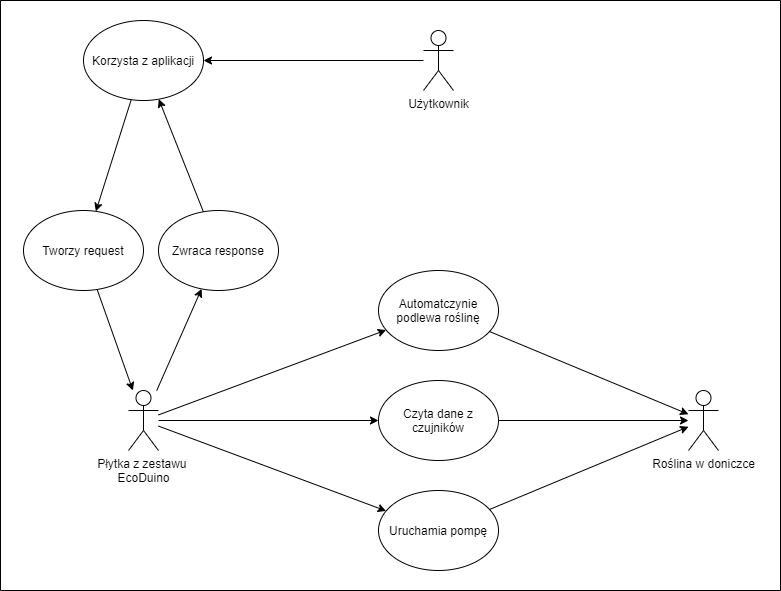
\includegraphics[width=\textwidth]{./assets/img/img001.png}
   \caption{Model UML przypadków użycia.}
   \label{fig:1}
\end{figure}

Do przeprowadzenia walidacji poprawności działania systemu został użyty Serial Port Monitor w Arduino IDE, testy jednostkowe aplikacji dekstop'owej oraz testy manualne całości. Fizycznie do testów, w pierwszej kolejności zostało użyte napełnione wodą pudełko, a finalnie roślina doniczkowa, aby zweryfikować działanie na prawdziwym przypadku użycia.

\section{Metodyka pracy nad projektowaniem i implementacją}

Podczas pracy nad projektem została użyta metodyka Kanban, której głównym celem jest wizualizacja procesu wykonywania danego projektu. Aby skorzystać z wyżej wspomnianej metodyki, należy przygotować fizyczną lub wirtualną tablicę z minimum 3 kolumnami (``To do'', ``In progress'' i ``Done''), oraz karteczkami opisującymi poszczególne etapy/zadania projektu. Dane karteczki zostają przekładane z jednej kolumny na kolejną wraz z postępami.

\begin{figure}[H]
   \centering
   \includegraphics[width=\textwidth]{./assets/img/img002.jpg}
   \caption{Metodyka pracy nad projektem.}
   \label{fig:2}
\end{figure}

Projekt został zaplanowany według wyżej wspomnianej metodyki i realizowany małymi etapami (Rysunek \ref{fig:2}). Nowe zadania zostały na bieżąco dodawane do kolumny ``To do'' w miarę rozwoju projektu. Pierwszymi zakończonymi etapami były analiza tematu, wraz z zebraniem wszelkich informacji i poszerzenia aktualnego stanu wiedzy o danym problemie i jego rozwiązaniach. Kolejnym etapem był zakup zestawu EcoDuino oraz przetestowanie jego modułów w celach weryfikacji działania, a także zdobycia wiedzy w jaki sposób użyć danych modułów. Następnie zostały stworzone puste projekty, osobno dla programu płytki z zestawu EcoDuino oraz aplikacji desktop'owej, a także nauka nowej technologii. Kolejnym krokiem było stworzenie kilku prostych widoków w aplikacji Flutter'owej, a także zastanowienie się nad składnią w żądaniach i zwrotkach w komunikacji w systemie. Po przemyśleniu wyżej wspomnianego problemu został przygotowany i przetestowany za pomocą Serial Port Monitor'u program obsługujący kilka podstawowych request'ów takich jak odczyt danych z sensorów lub uruchomienie i zatrzymanie pompy. Następnie zostały przygotowane widoki w aplikacji desktop'owej do obsługi tych request'ów. Została dodana nowa funkcjonalność automatycznego podlewania po stronie programu na płytce jak i w aplikacji desktop'owej, po czym został przetestowany cały system. Podczas realizacji projektu zostały napotkane różne problemy, które zostały wyznaczone jako osobne zadania i w późniejszym czasie realizacji projektu zostały one naprawione. Jednym z największych problemów był problem związany z asynchronicznością aplikacji przy jednoczesnym odczytywaniu kilku czujników w tym samym czasie. Został on naprawiony wydzieleniem każdego żądania do osobnego wątku aplikacji.

\section{Wykorzystane narzędzia i technologie}

Podczas tworzenia projektu zostały użyte narzędzia i technologie przedstawione poniżej:

\begin{itemize}
   \item	Arduino - język programowania pozwalający tworzyć oprogramownie na różne płytki Arduino, jest bazujący na Wiring oraz C++, został zapoczątkowany w 2005 roku,
   \item Arduino IDE - środowisko programistyczne dla języka programowania Arduino, pozwala ono między innymi na napisanie kodu programu, pobranie dodatkowych bibliotek z repozytorium, kompilacje, wgranie programu na płytkę, wypalenie bootloader'a oraz użycie Serial Port Monitor'a,
   \item Flutter - zestaw narzędzi dla języka programowania Dart, pozwalających na napisanie natywnej, wieloplatformowej aplikacji z nowoczesnym design'em, został stworzony w 2017 roku przez firmę Google,
   \item Dart - język programowania cechujący się obiektowością, posiadaniem garbage collector'a, kompilacją zarówno do kodu natywnego, a także do JavaScript'u, został on stworzony w 2013 roku przez firmę Google,
   \item Visual Studio Code - edytor kodu źródłowego stworzony przez firmę Microsoft w roku 2015, posiada w sobie wiele wbudowanych funkcjonalności, między innymi podpowiadanie składni kodu, refaktoryzacja, debugger, kolorowanie składni i inne, dodatkowo można dodać nowe funkcjonalności instalując rozszerzenia. W projekcie został użyty do stworzenia aplikacji desktop'owej w Flutter'ze, dodatkowo została użyta wtyczka ``Dart-Code.flutter'',
   \item Windows 11 - system operacyjny stworzony przez firmę Microsoft w 2021 roku, został on wykorzystany podczas całego procesu tworzenia projektu i pracy dyplomowej, aplikacja na płytkę oraz aplikacja desktop'owa zostały skompilowane na tym systemie,
   \item diagrams.net - narzędzie do tworzenia diagramów UML, poprzednio nazywane było draw.io. Narzędzie zostało wykorzystane do utworzenia diagramu przypadków użycia,
   \item PlantUML - narzędzie do tworzenia diagramów UML przy użyciu napisanego kodu, zostało stworzone w 2009 roku przez Arnaud Roques'a. Narzędzie zostało wykorzystane przy tworzeniu diagramów UML klas, zarówno w programie na płytkę z zestawu EcoDuino, a także w aplikacji desktop'owej,
   \item hpp2plantuml - narzędzie konsolowe pozwalające wygenerować kod diagramu UML dla narzędzia PlantUML z plików języka C++. Narzędzie zostało wykorzystane do utworzenia diagramu klas  w programie na płytkę z zestawu EcoDuino,
   \item dcdg - narzędzie konsolowe, napisane w języku Dart, pozwalające wygenerować kod diagramu UML dla narzędzia PlantUML z plików języka Dart. Narzędzie zostało wykorzystane do utworzenia diagramu klas aplikacji desktop'owej.

\end{itemize}

\chapter{Specyfikacja zewnętrzna}

W tym rozdziale ukazana jest specyfika zewnętrzna projektu, tzn. przedstawione są wymagania zarówno sprzętowe jak i programowe, schemat płytki, diagram zestawu EcoDuino, a także ukazany jest sposób instalacji poszczególnych części zestawu oraz instalacja programu na płytkę czy też aplikacji desktop'owej. Dodatkowo opisany jest sposób obsługi, kwestie bezpieczeństwa, a także przykładowy scenariusz działania.

\section{Wymagania sprzętowe i programowe}

Wymagania sprzętowe i programowe dla danego projektu jakie trzeba spełnić to:

\begin{itemize}
   \item posiadanie zestawu EcoDuino,
   \item posiadanie komputera z zainstalowanym systemem Windows 7 SP1 lub nowszy \cite{bib:url001},
   \item opcjonalnie posiadanie 6 baterii AA lub zasilacza DC 6-12V w celu zasilenia zestawu EcoDuino oraz pompy (sam zestaw EcoDuino można alternatywnie zasilić przy użyciu przewodu microUSB, ale pompa potrzebuje już większego zasilania).
\end{itemize}

Wykorzystany w projekcie zestaw EcoDuino składa się z kilku elementów, w których skład wchodzą:

\begin{itemize}
   \item płytka główna FreeLife bazująca na Arduino Leonardo, posiadająca:
         \begin{itemize}
            \item mikrokontroler ATmega 32u4,
            \item 5 pinów cyfrowych I/O,
            \item 4 wejścia analogowe,
            \item gniazdo do czujnika wilgotności,
            \item gniazdo do podłączenia pompy,
            \item gniazdo do podłączenia modułu komunikacji Xbee,
            \item gniazdo micro USB,
         \end{itemize}
   \item pompa o parametrach:
         \begin{itemize}
            \item napięcie zasilania pompy 4.5V - 12V,
            \item moc maksymalnie 5W,
            \item przepływ 100 - 350 L/H,
         \end{itemize}
   \item obudowa do płytki,
   \item czujnik wilgotności gleby,
   \item czujnik temperatury i wilgotności powietrza DHT11,
   \item wężyk do wody,
   \item koszyk na 6 baterii AAA,
   \item przewód microUSB,
   \item dwa śrubokręty,
   \item gniazdo DC,
   \item zestaw przewodów.
\end{itemize}

\section{Schemat płytki}

Schemat płytki z zestawu EcoDuino został przedstawiony na rysunku \ref{fig:3}.

\begin{figure}[H]
   \centering
   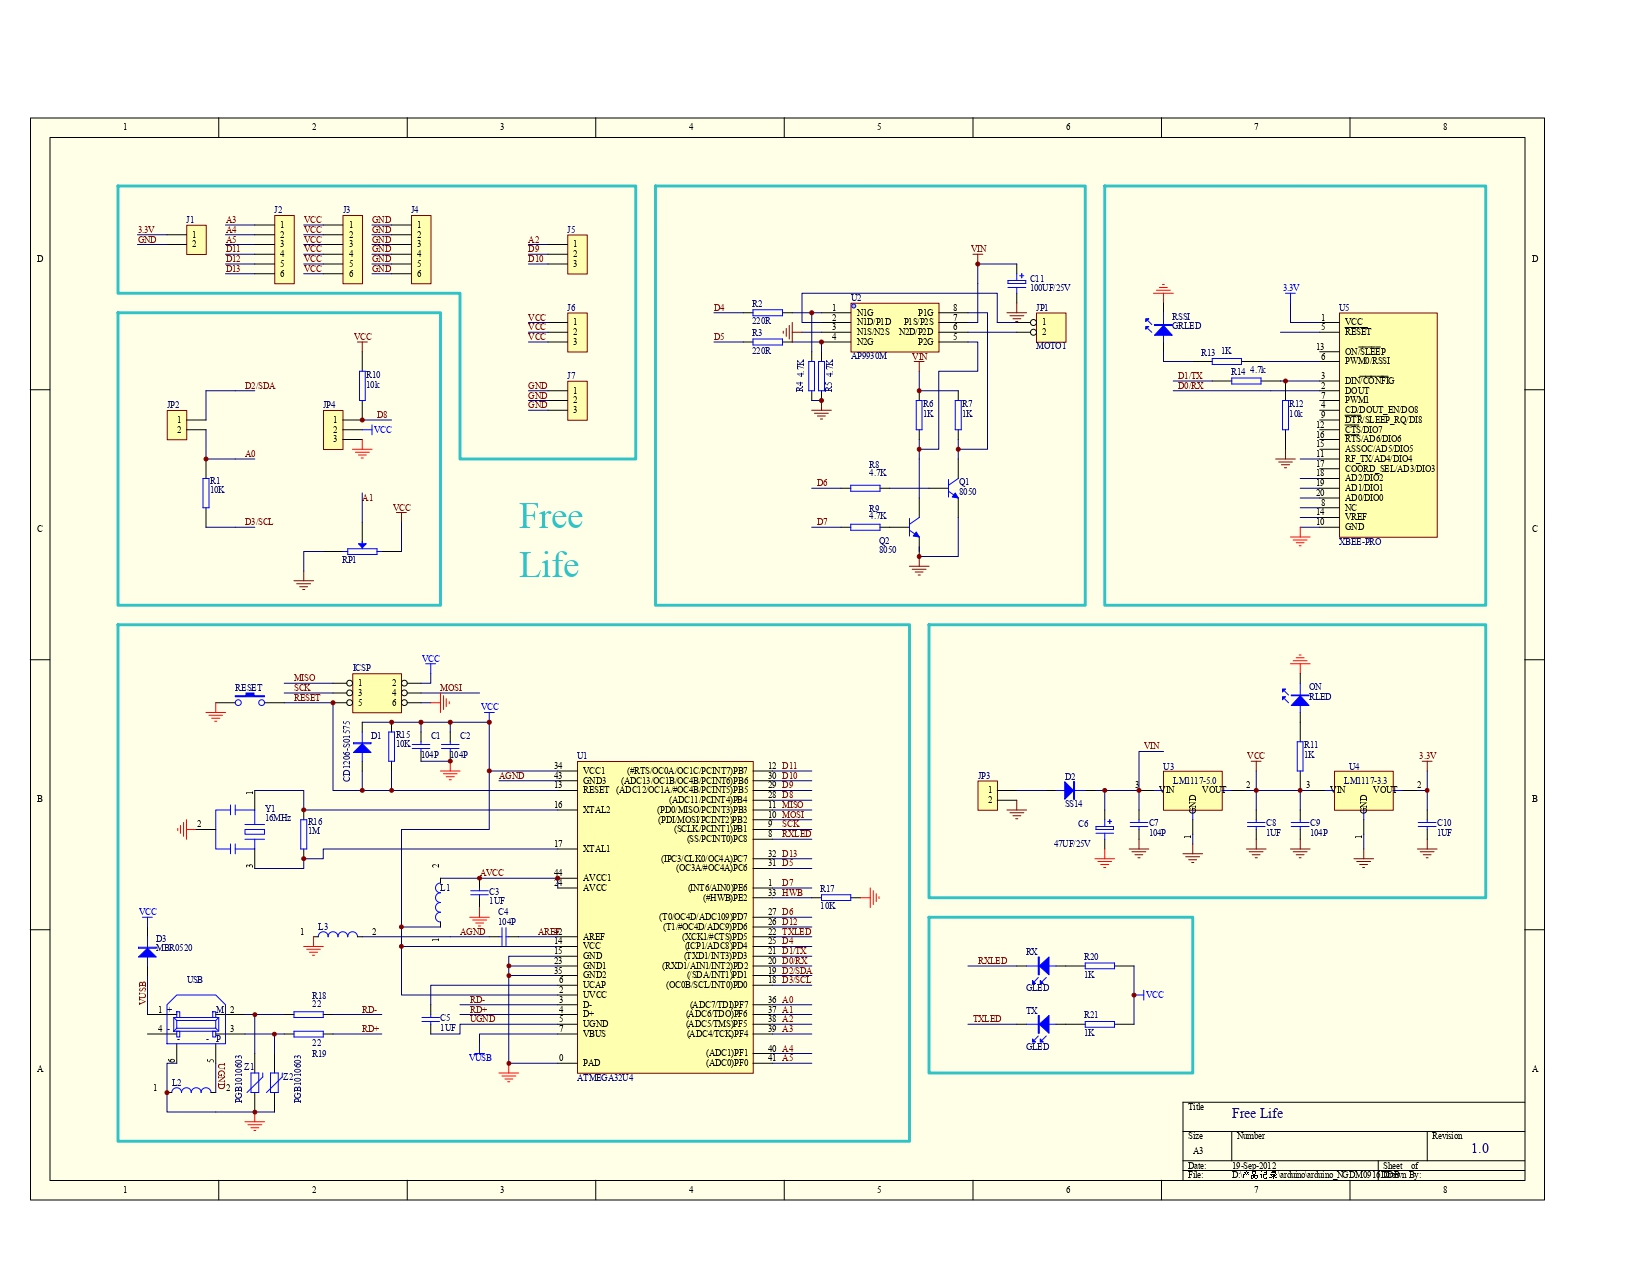
\includegraphics[width=\textwidth]{./assets/img/img003.jpg}
   \caption{Schemat płytki. \cite{bib:url002}}
   \label{fig:3}
\end{figure}

\newpage

\section{Diagram zestawu EcoDuino}

Diagram zestawu EcoDuino został przedstawiony na rysunku \ref{fig:4}.

\begin{figure}[H]
   \centering
   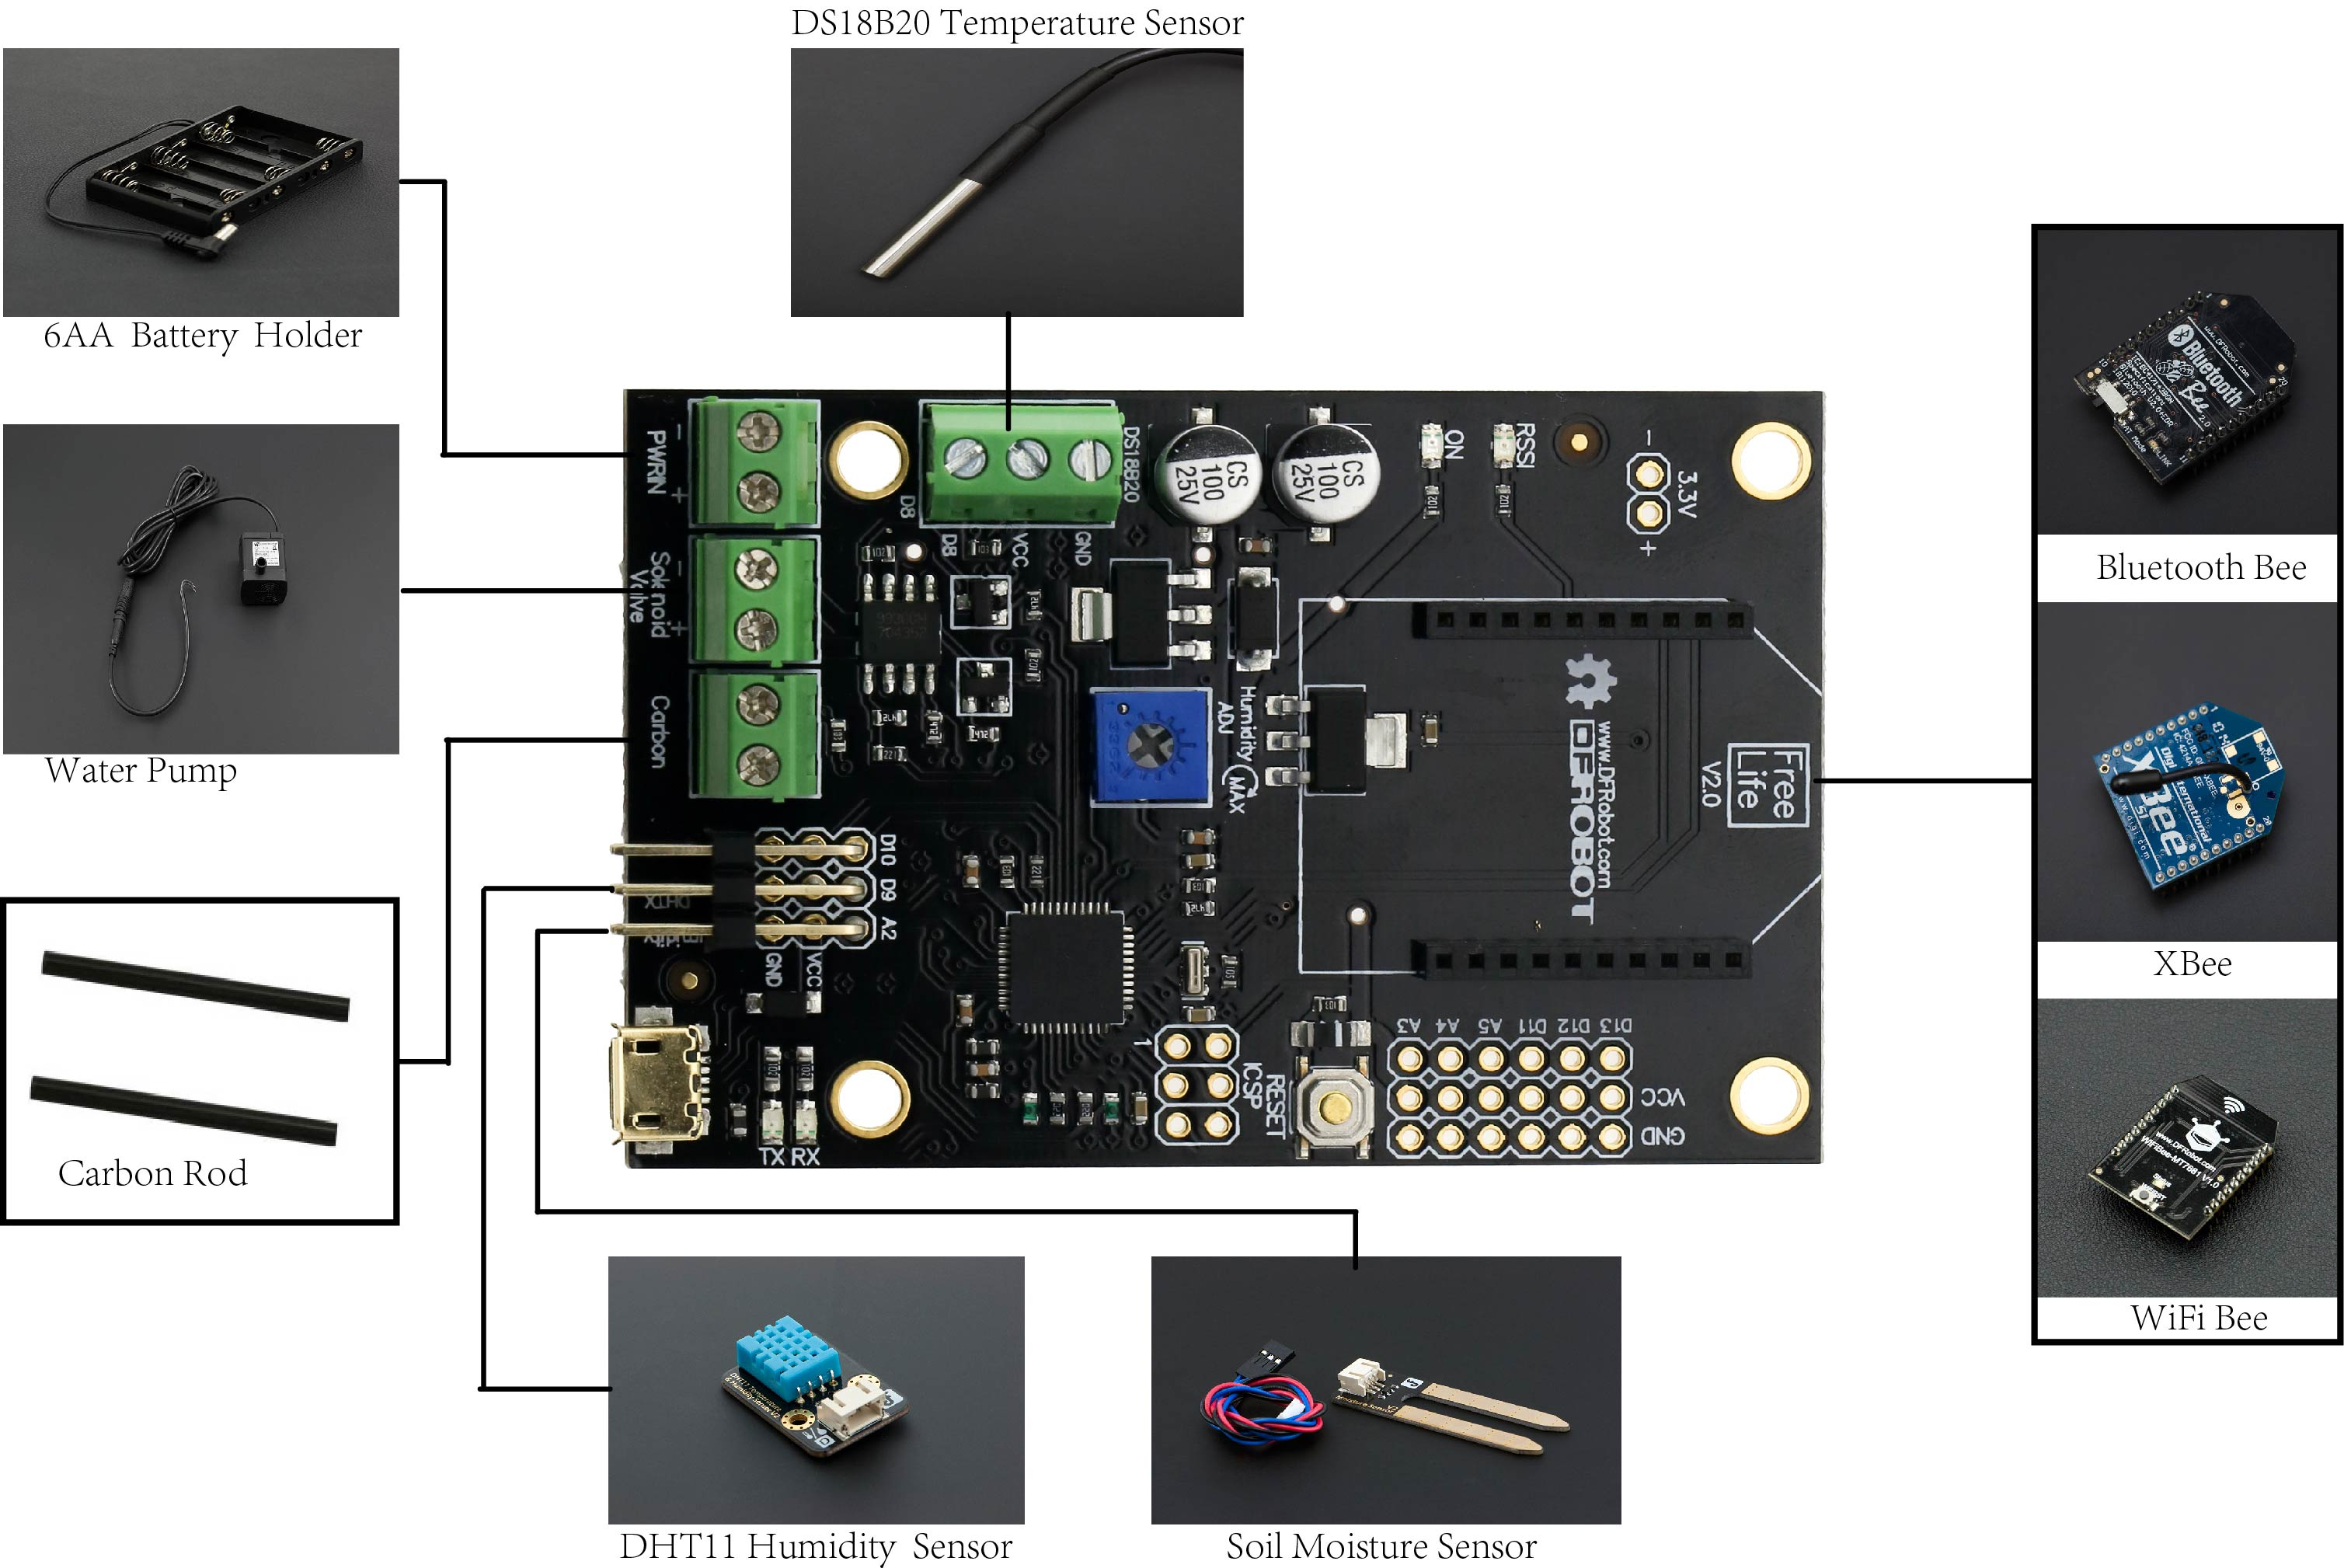
\includegraphics[width=\textwidth]{./assets/img/img004.jpg}
   \caption{Diagram zestawu EcoDuino. \cite{bib:url003}}
   \label{fig:4}
\end{figure}

\newpage

\section{Sposób instalacji}

Aby zestaw EcoDuino działał, należy najpierw podłączyć prawidłowo wszystkie przewody, kolejność obojętna (Rysunek \ref{fig:5}).

\begin{figure}[H]
   \centering
   \includegraphics[width=\textwidth]{./assets/img/img005.jpg}
   \caption{Podłączenie przewodów na płytce.}
   \label{fig:5}
\end{figure}

\newpage

Aby podłączyć czujnik temperatury i wilgotności powietrza DHT11 należy wykorzystać jeden z dostępnych w zestawie przewodów, w projekcie został użyty czarno-czerwono-zielony. Pierwszy pin należy podpiąć pod digital'owy pin D9 na płytce, drugi pod VCC, a trzeci pod GND (Rysunek \ref{fig:6}).

\begin{figure}[H]
   \centering
   \includegraphics[width=\textwidth]{./assets/img/img006.jpg}
   \caption{Podłączenie przewodu pod czujnik temperatury i wilgotności powietrza.}
   \label{fig:6}
\end{figure}

\newpage

Kolejnym elementem jest czujnik wilgotności gleby i aby podłączyć należy wykorzystać drugi z dostępnych w zestawie przewodów, na rzecz projektu został użyty przewód czarno-czerwono-niebieski. Pierwszy pin w czujniku należy podpiąć do analogowego pinu A2, drugi pod VCC, a trzeci pod GND (Rysunek \ref{fig:7}).

\begin{figure}[H]
   \centering
   \includegraphics[width=\textwidth]{./assets/img/img007.jpg}
   \caption{Podłączenie przewodu pod czujnik temperatury.}
   \label{fig:7}
\end{figure}

Następnym użytym elementem jest pompa, która jest podłączona do ``Soneloid Valve'' odpowiednio brązowym przewodem do ``+'' i niebieskim do ``-''. Przewód został przykręcony dołączonym do zestawu śrubokręty krzyżykowym.

Ostatnim elementem jest przewód z gniazdem DC, który jest podłączony do ``PWRN'' odpowiednio czerwonym przewodem do ``+'' i czarnym do ``-''. Przewód ten, jak powyżej także został przykręcony śrubokrętem.

Na płytkę został wgrany odpowiednio przygotowany wcześniej program, który zostaje uruchomiony zaraz po podłączeniu źródła prądu. Aplikacja desktop'owa, po uprzednim zbudowaniu, nie wymaga żadnych dodatkowych kroków podczas uruchomienia.

Aby zainstalować program na płytkę z zestawu EcoDuino należy zainstalować Arduino IDE, otworzyć kod programu ``ecoduino.ino'', wybrać z paska menu głównego opcję ``Tools'' \textrightarrow  ``Board'' \textrightarrow  ``Arduino Leonardo'' (Rysunek \ref{fig:8}) oraz port w ``Tools'' \textrightarrow  ``Port'' \textrightarrow  ``Wybrać odpowiedni port'' (na przykład ``COM6'').

\begin{figure}[H]
   \centering
   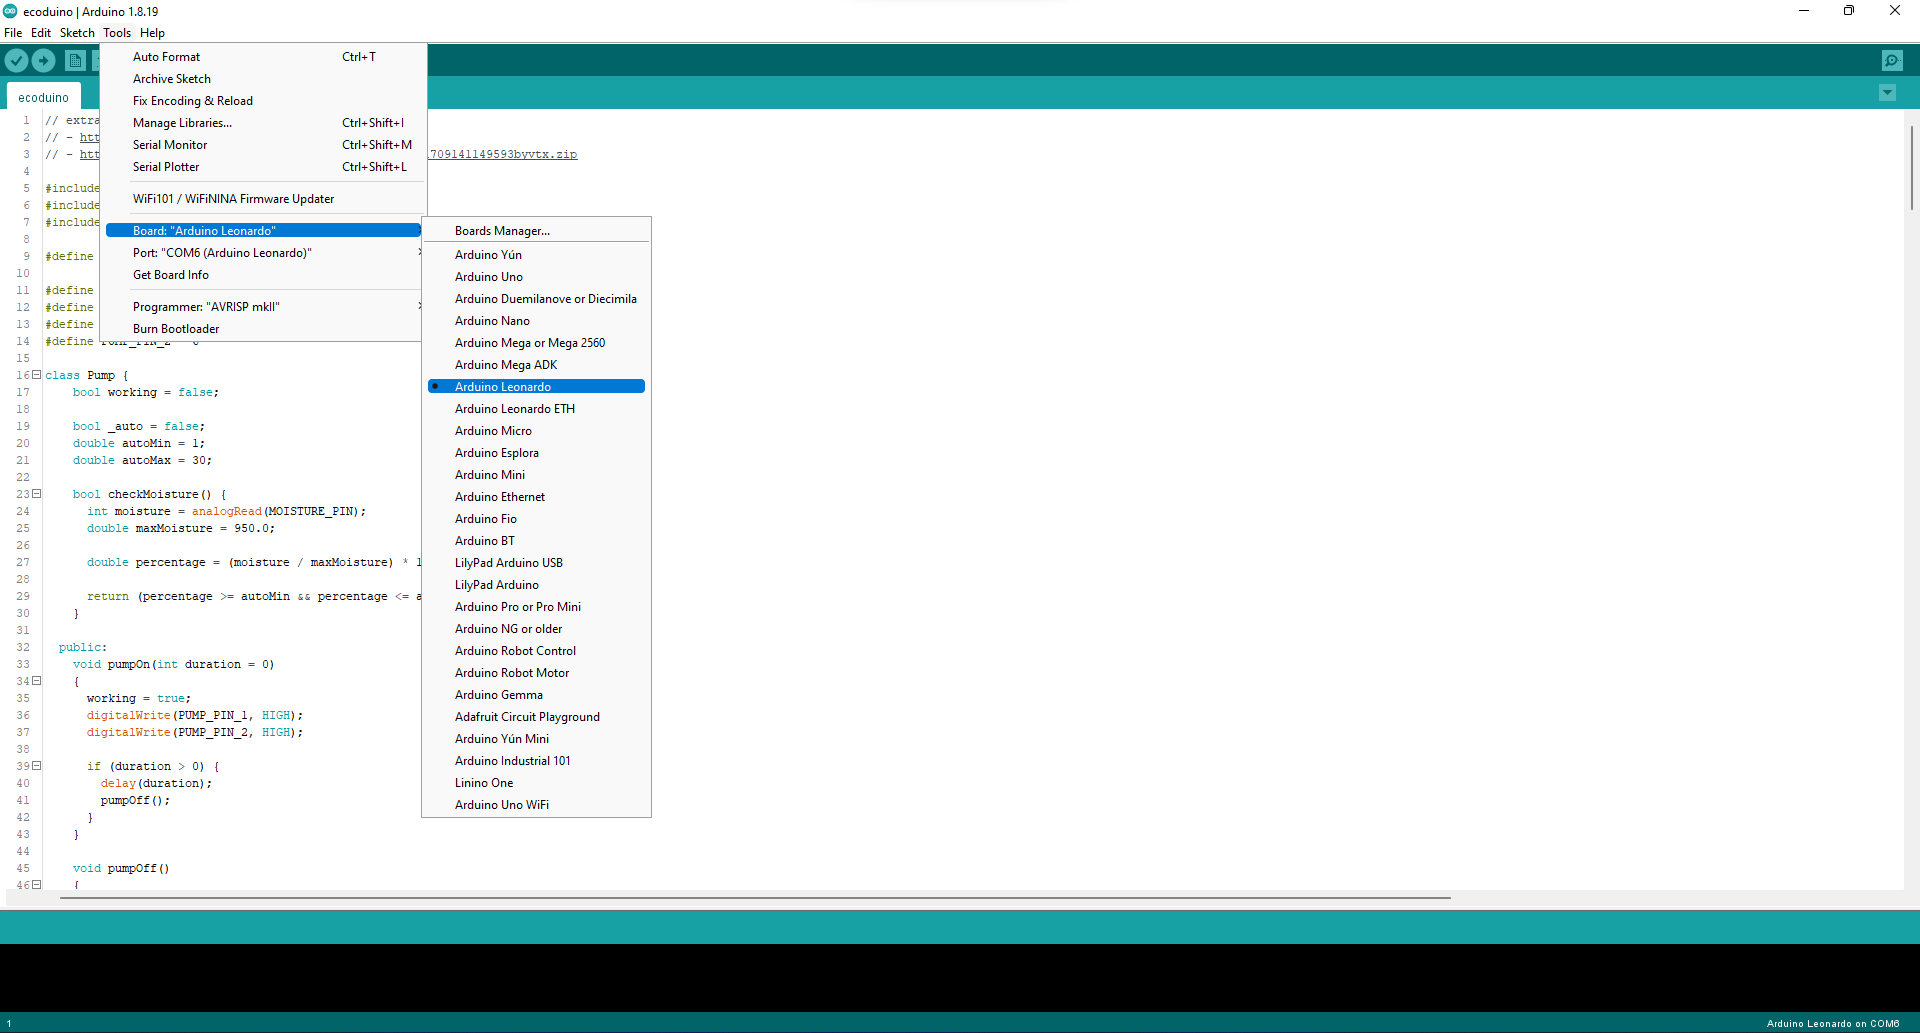
\includegraphics[width=\textwidth]{./assets/img/img008.png}
   \caption{Ustawienie płytki w Arduino IDE.}
   \label{fig:8}
\end{figure}

\newpage

Następnie należy doinstalować biblioteki ``nickgammon/Regexp'' i ``DHT11''. Aby zainstalować bibliotekę ``Regexp'' należy wybrać z paska menu głównego ``Tools'' \textrightarrow  ``Manage libraries...'', wyszukać frazę ``Regexp'' i zainstalować paczkę (Rysunek \ref{fig:9}). Aby zainstalować paczkę ``DHT11'' należy pobrać ją z linku na początku kodu źródłowego pliku ``ecoduino.ino'' \cite{bib:url004}, rozpakować paczkę i przenieść do folderu ``C:\textbackslash Users\textbackslash \textless nazwa\_uzytkownika\textgreater \textbackslash Documents\textbackslash Arduino\textbackslash Libraries''. Po tych akcjach obie biblioteki będą dostępne w środowisku.

\begin{figure}[H]
   \centering
   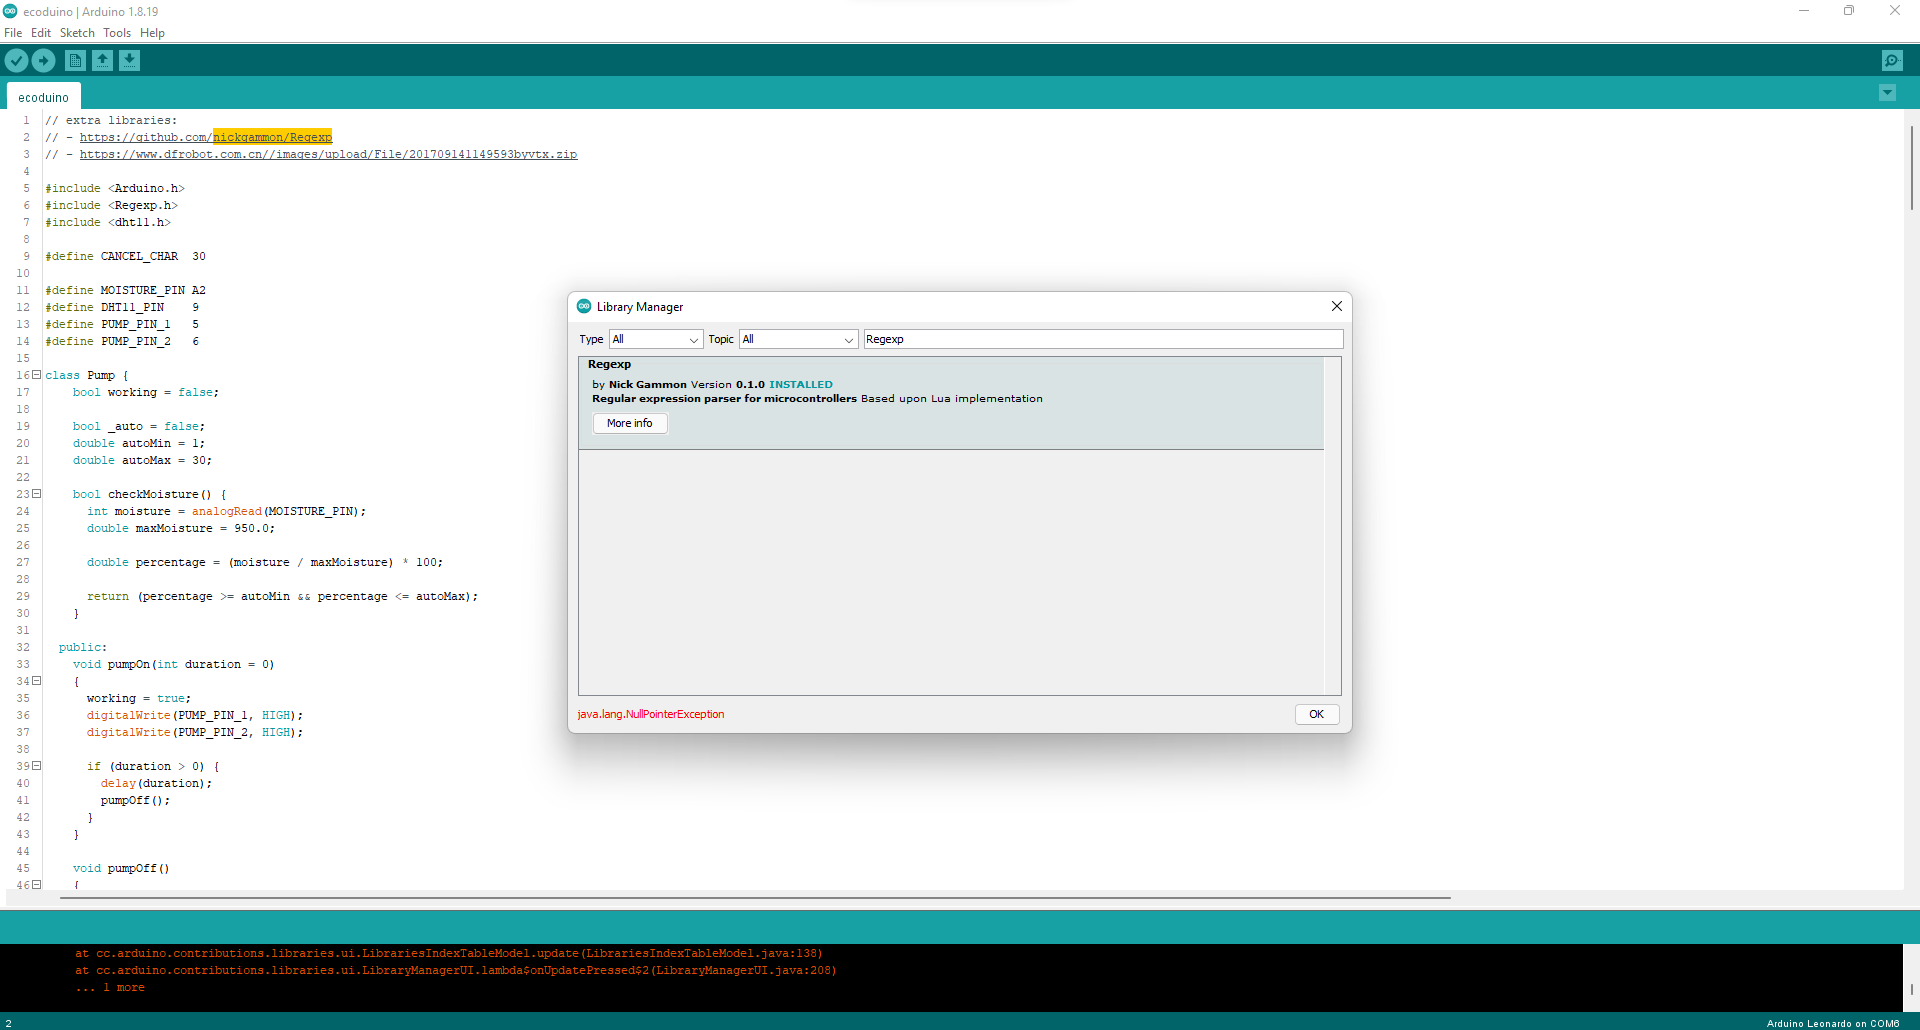
\includegraphics[width=\textwidth]{./assets/img/img009.png}
   \caption{Instalacja biblioteki ``Regexp''.}
   \label{fig:9}
\end{figure}

Kolejnym krokiem jest wybranie przycisku ``Verify'' z górnej belki w celu weryfikacji i kompilacji kodu, a następnie ``Upload'' w celu posłania skompilowanego programu na płytkę z zestawu EcoDuino.

Aby zbudować aplikację desktop'ową należy zainstalować Flutter'a korzystając z oficjalnej dokumentacji \cite{bib:url005}. W pierwszym kroku należy pobrać ukazaną paczkę z najnowszym Flutter SDK i rozpakować ją w wybranym miejscu oraz dodać folder ``flutter\textbackslash bin'' do zmiennej środowiskowej ``PATH''. Po tej akcji w konsoli PowerShell powinno być dostępne polecenie ``flutter'', dzięki czemu możemy już korzystać z wszystkich jego możliwości. Aby dokończyć instalacje należy w konsoli PowerShell wykonać komendę ``flutter doctor'', zainstaluje ona wszystkie zależności dla platformy oraz wyświetli raport statusu instalacji Flutter'a. Aby aplikacja działała na Windows'ie należy dodatkowo zainstalować Visual Studio 2019 oraz podczas instalacji wybrać paczkę ``Desktop development with C++'', a następnie w konsoli wykonać komendę ``flutter config \texttt{-{}-}enable\texttt{-}windows\texttt{-}desktop''. Po wykonanych akcjach można zweryfikować czy instalacja została wykonana pomyślnie wykonując polecenie ``flutter doctor'' i oberwawszy brak błędu dla środowiska Windows (Rysunek \ref{fig:10}).

\begin{figure}[H]
   \centering
   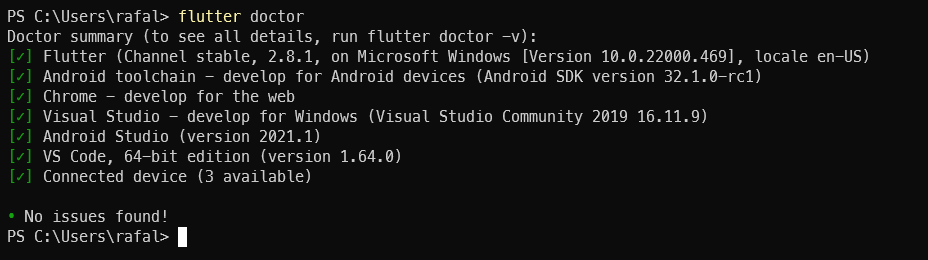
\includegraphics[width=\textwidth]{./assets/img/img010.png}
   \caption{Wykonanie polecenia ``flutter doctor''.}
   \label{fig:10}
\end{figure}

Aby zbudować aplikację należy wykonąc polecenie ``flutter build windows'' (Rysunek \ref{fig:11}). Dzięki tej komendzie zostanie zbudowana finalna aplikacja i będzie ona dostępna w podkatalogu projektu ``build\textbackslash windows\textbackslash runner\textbackslash Release\textbackslash nazwa\_projektu.exe'' (Rysunek \ref{fig:12}).

\begin{figure}[H]
   \centering
   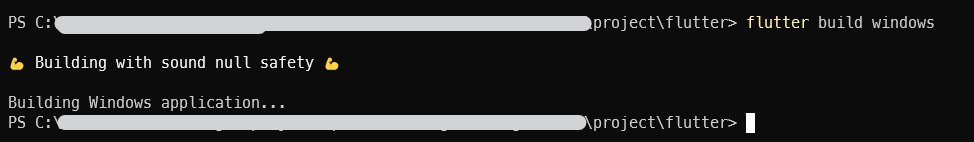
\includegraphics[width=\textwidth]{./assets/img/img011.png}
   \caption{Wykonanie polecenia ``flutter build windows''.}
   \label{fig:11}
\end{figure}

\begin{figure}[H]
   \centering
   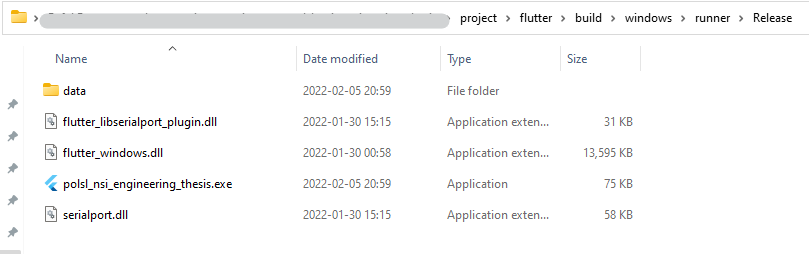
\includegraphics[width=\textwidth]{./assets/img/img012.png}
   \caption{Przedstawiona finalna lokalizacja aplikacji.}
   \label{fig:12}
\end{figure}

Po uruchomieniu finalnego pliku, ukazuje się ekran startowy aplikacji (Rysunek \ref{fig:13}).

\begin{figure}[H]
   \centering
   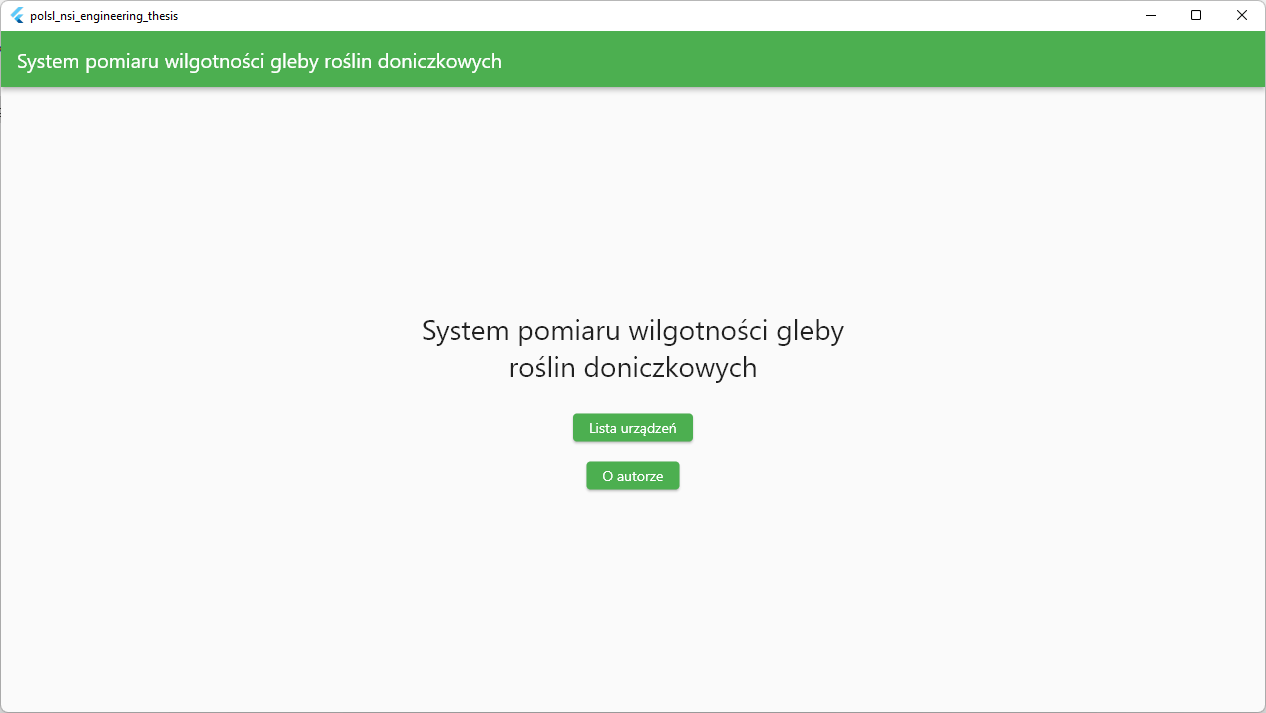
\includegraphics[width=\textwidth]{./assets/img/img013.png}
   \caption{Ekran startowy aplikacji.}
   \label{fig:13}
\end{figure}

\section{Sposób aktywacji}

Po instalacji programu na płytkę oraz aplikacji desktop'owej system jest gotowy do użytku. Należy podłączyć urządzenie do prądu, uruchomić aplikację na komputerze i podpiąć kabel microUSB do urządzenia. Po wykonaniu tych czynności, w aplikacji na liście urządzeń powinno pojawić się nowe urządzenie, ewentualnie należy odświeżyć widok (Rysunek \ref{fig:14}).

\begin{figure}[H]
   \centering
   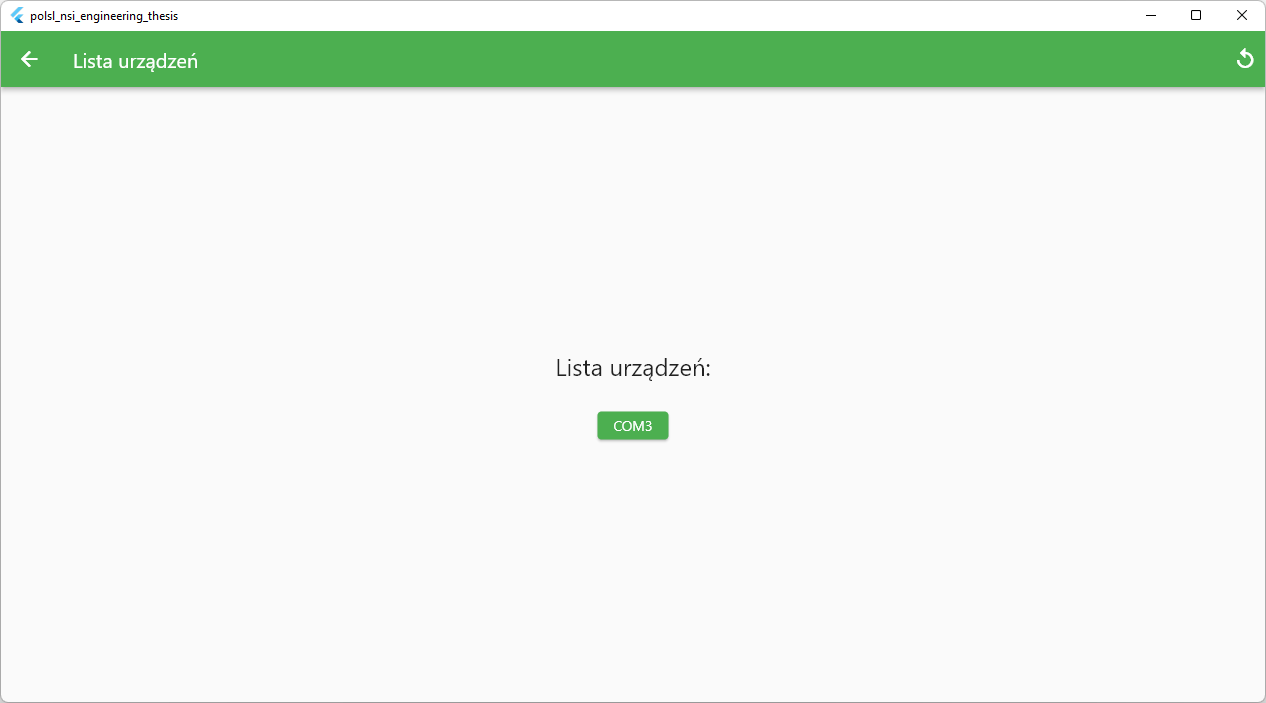
\includegraphics[width=\textwidth]{./assets/img/img014.png}
   \caption{Lista dostępnych urządzeń.}
   \label{fig:14}
\end{figure}

\newpage

Po wybraniu urządzenia dostępna już jest możliwość jego zarządzania (Rysunek \ref{fig:15}).

\begin{figure}[H]
   \centering
   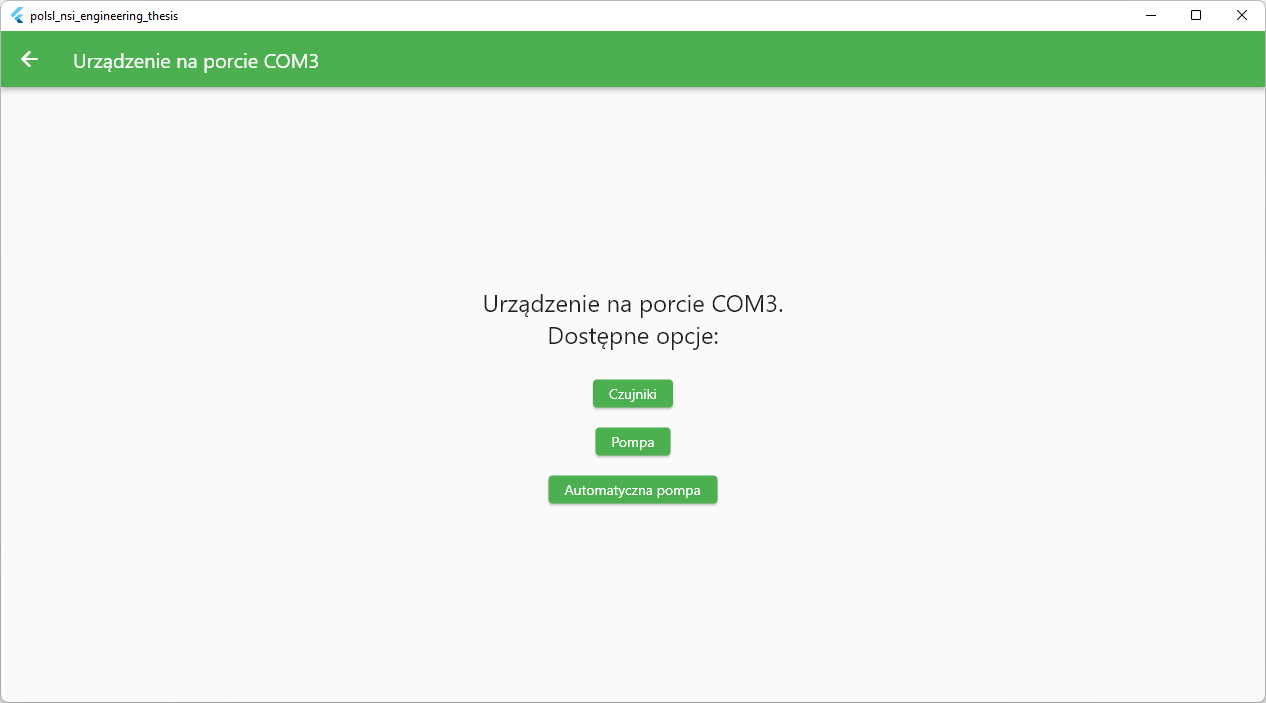
\includegraphics[width=\textwidth]{./assets/img/img015.png}
   \caption{Zarządzanie urządzeniem.}
   \label{fig:15}
\end{figure}

\section{Sposób obsługi}

Do zarządzania urządzeniem dostępne są trzy opcje:

\begin{itemize}
   \item ``Czujniki'' - monitorowanie czujników urządzenia,
   \item ``Pompa'' - włączanie/wyłączanie pompy,
   \item ``Automatyczna pompa'' - włączanie/wyłączanie automatycznego podlewania rośliny, a także ustawienie zakresu wilgotności gleby w jakim pompa ma zostać aktywowana.
\end{itemize}

\newpage

W widoku ``Czujniki'' możliwe jest monitorowanie podłączonych czujników (Rysunek \ref{fig:16}). Dostępne są 3 okrągłe wskaźniki:

\begin{itemize}
   \item dla czujnika wilgotności gleby,
   \item dla czujnika wilgotności powietrza,
   \item dla czujnika temperatury.
\end{itemize}

Każdy z nich, poza temperaturą, wskazuje procentowe dane sczytane z czujnika z dokładnością do 2 miejsc po przecinku. W przypadku czujnika temperatury okrągły wskaźnik reprezentuje procentowe dane aktualnej temperatury względem minimalnej i maksymalnej wartości jakie mogą być sczytane używając tego czujnika, a liczba w środku podaje aktualną temperaturę otoczenia w stopniach Celsiusza.

W przypadku niedostępności któregoś z czujników pojawia się tekst ``N/A'', a okrągły wskaźnik kręci się w kółko (Domyślne zachowanie ``CircularProgressIndicator'' w Flutter'ze gdy wartość jest równa 0).

\begin{figure}[H]
   \centering
   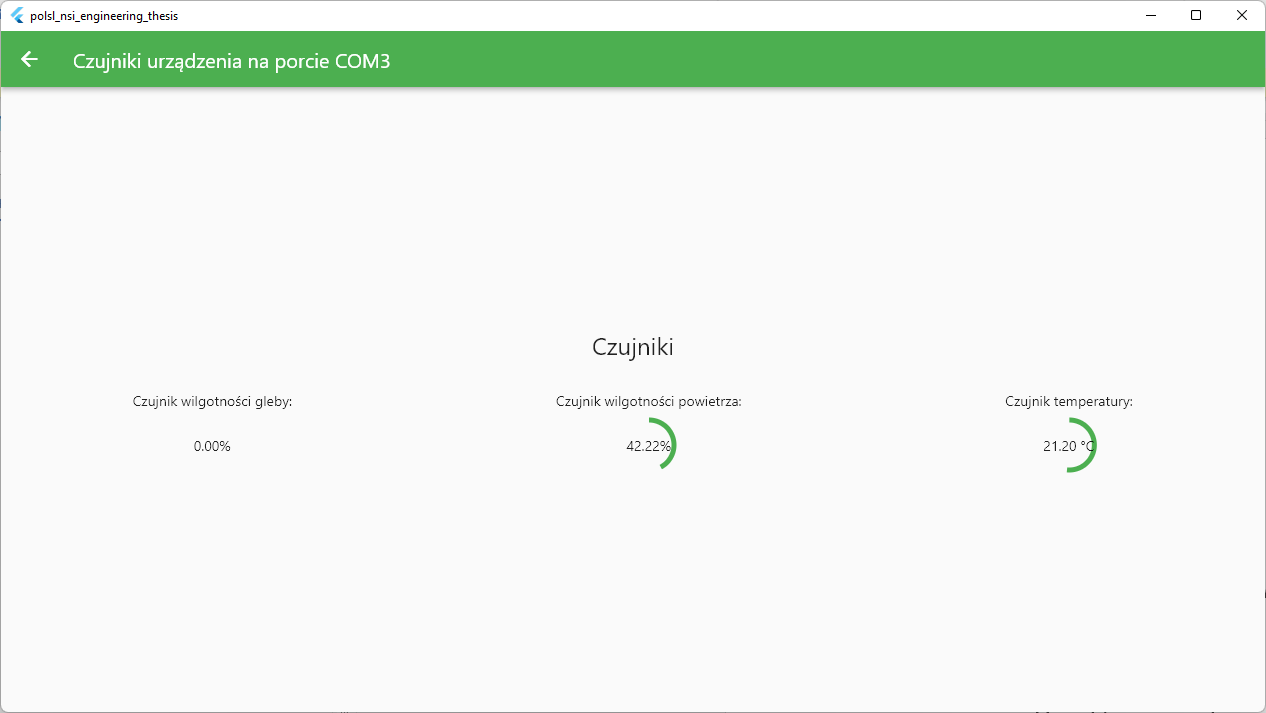
\includegraphics[width=\textwidth]{./assets/img/img016.png}
   \caption{Widok czujników urządzenia.}
   \label{fig:16}
\end{figure}

Kolejnym widokiem jest widok nazwany ``Pompa'' i posiada on jeden przycisk, który pozwala na manualne włączenie i wyłączenie pompy (Rysunek \ref{fig:17}). Dodatkowo po kliknięciu przycisku ``Start'' zmienia on nazwę na ``Stop'', a także zmienia kolor na czerwony, a po ponownym kliknięciu tekst zmienia się z powrotem na ``Start'', a kolor na domyślny aplikacji.

\begin{figure}[H]
   \centering
   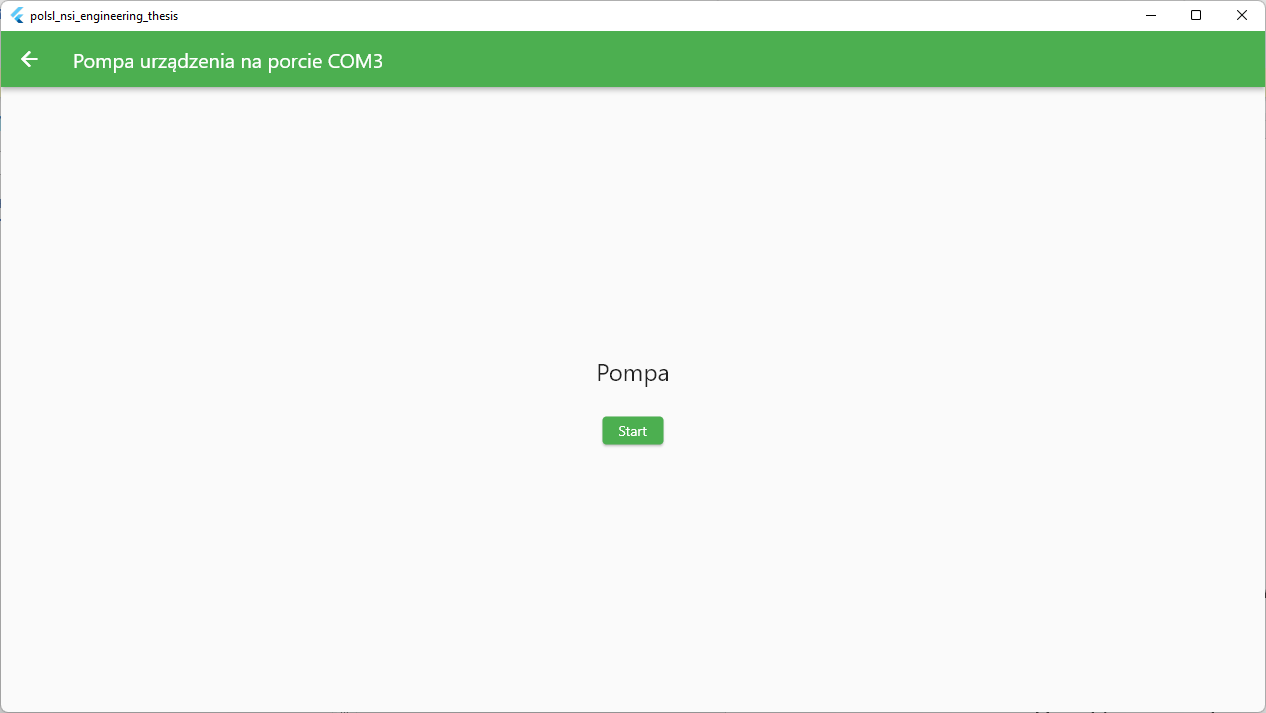
\includegraphics[width=\textwidth]{./assets/img/img017.png}
   \caption{Widok pompy.}
   \label{fig:17}
\end{figure}

Ostatnim widokiem jest widok nazwany ``Automatyczne podlewanie'' (Rysunek \ref{fig:18}) i posiada on dwie opcje:

\begin{itemize}
   \item włączenie/wyłączenie funkcji automatycznego podlewania,
   \item ustawienie zakresu wilgotności gleby w jakiej pompa ma zostać włączona.
\end{itemize}

Cała funkcjonalność zaczyna działać dopiero po włączenia jej używając checkbox'a. Poniżej znajdujący się suwak z zakresem pozwala wyznaczyć procentową, początkową i końcową wartość czujnika wilgotności gleby, po której osiągnięciu powinna uruchomić się pompa. Wartości te są w zakresie 1-100 i suwakiem można poruszać o 1 jednostkę. Podane ograniczenia zakresu, zaczynające się od 1 wynikają z powodu uniknięcia sytuacji, w której pompa zaczyna działać po wyciągnięciu czujnika wilgotności gleby z rośliny.

\begin{figure}[H]
   \centering
   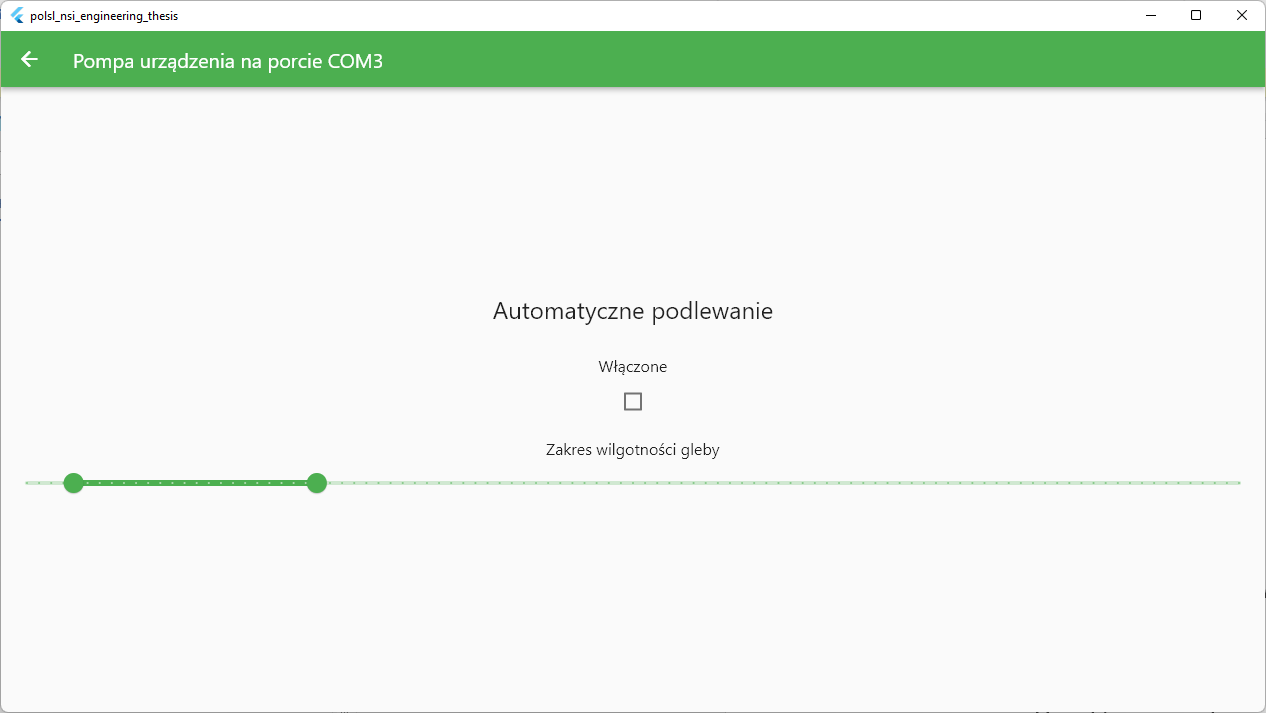
\includegraphics[width=\textwidth]{./assets/img/img018.png}
   \caption{Widok automatycznego podlewania.}
   \label{fig:18}
\end{figure}

\section{Administracja systemu}

Administratorem systemu zostaje końcowy użytkownik korzystający z danego systemu. Został on stworzony w taki sposób, aby użytkownik mógł w prosty i przejrzysty sposób monitorować stan wilgotności gleby i czynników na około rośliny oraz podlewać manualnie i automatycznie roślinę.

\section{Kwestie bezpieczeństwa}

Od kwestii fizycznej projektu należy zwrócić szczególną uwagę na ustawienie urządzenia i zbiornika z wodą, w którym zanurzona jest pompa, aby nie przewrócić całego zestawu, pomyłkowo zahaczając o na przykład rurkę z pompy, co może spowodować zalanie niżej znajdujących się rzeczy.

Kolejną rzeczą na jaką warto zwrócić uwagę jest monitorowanie poziomu wody w zbiorniku gdzie jest umieszczona pompa. Zbyt mała ilość może spalić mechanizm pompy i spowodować permanentne uszkodzenie pompy.

Od kwestii programowej, całość zarządzania urządzeniem dzieje się poprzez użycie przewodu microUSB, dzięki czemu pozostaje wyeliminowane wykorzystanie urządzenia przez niepowołane osoby z zewnątrz, ponieważ do skorzystania z urządzenia jest potrzebny do niego fizyczny dostęp.

\section{Przykład działania}

Przykładowy scenariusz działania aplikacji wygląda następująco:

Użytkownik otrzymuje wcześniej przygotowany i złożony zestaw oraz archiwum zip z zbudowaną aplikacją desktop'ową. Po rozpakowaniu zestawu użytkownik wkłada czujnik wilgotności do rośliny, przygotowuje źródło wody i wkłada do niego pompę używając dostępnych w pompie przyssawek, oraz podpina urządzenie do źródła zasilania. Następnie rozpakowuje paczkę zip z aplikacją desktop'ową, podłącza komputer do urządzenia kablem microUSB i korzysta z aplikacji, na przykład sprawdzając status czujników i ustawiając automatyczne podlewanie rośliny. Po wykonaniu wszystkich czynności, użytkownik odłącza kabel. Gdy użytkownik chce zakończyć działanie urządzenia, odłącza je od źródła zasilania.

Alternatywnie użytkownik otrzymuje zestaw EcoDuino do samodzielnego złożenia oraz otrzymuje kod programu na płytkę, a także kod aplikacji desktop'owej i instrukcję instalacji i aktywacji. Użytkownik składa urządzenie przy użyciu informacji z punktu 4.4 i 4.5. Po przygotowaniu do użytku zestawu, użytkownik może rozpocząć pracę tak jak zostało to opisane w poprzednim scenariuszu.

\chapter{Specyfikacja wewnętrzna}

Poniższy rozdział obejmuje tematykę przedstawienia idei projektu, przedstawienia architektury sytemu jaka została użyta, wykonany został przegląd najważniejszych klas, modułów, komponentów i bibliotek. Dodatkowo zostały opisane szczegóły implementacji ważniejszych algorytmów oraz ważniejszych fragmentów kodu, zastosowane wzorce projektowe i diagramy UML klas.

\section{Przedstawienie idei}

Ideą było stworzenie systemu pozwalającego na szybkie podłączenie zestawu do rośliny oraz zaprogramowanie aplikacji do jej monitorowania i zarządzania z prostym i przyjaznym użytkownikowi interfejsem pozwalający użytkownikowi na najlepszy UX (ang. \textit{User eXperience}).

\section{Architektura systemu}

Architekturą wykorzystaną w systemie jest zmodyfikowana, uproszczona pod projekt wersja protokołu HTTP. Pojedyncze żądanie wygląda jak na kodzie \ref{code:1}.

\begin{figure}[H]
   \centering
   \footnotesize
   \begin{lstlisting}
      METODA /routing?parametr1=wartosc&parametr2=wartosc
   \end{lstlisting}
   \caption{Schemat pojedynczego żądania.}
   \label{code:1}
\end{figure}

\begin{itemize}
   \item METODA - jedna z 2 dostępnych w systemie metod:
         \begin{itemize}
            \item GET - służy do pobierania danych z urządzenia,
            \item POST - służy do zapisu danych na urządzeniu lub wykonaniu na nim jakiejś akcji,
         \end{itemize}
   \item	/routing - ścieżka do akcji jaka ma zostać wykonana, dostępne w systemie ścieżki to:
         \begin{itemize}
            \item /moisture - działa tylko z metodą GET, zwraca dane z czujnika wilgotności gleby, zwracane dane:
                  \begin{itemize}
                     \item value - wartość odczytana z czujnika,
                     \item min - minimalna wartość czujnika (0),
                     \item max - maksymalna wartość czujnika (950),
                     \item ranges - tablica z oznaczeniami poszczególnych zakresów, pojedynczy zakres składa się z 3 elementów: ``from'' - wartość początku zakresu, ``to'' - wartość końca zakresu, ``title'' - tytuł, oznaczenie danego zakresu. Zwracane są 3 elementy z zakresami i oznaczeniami takimi jak prezentuje dokumentacja \cite{bib:url006}:
                           \begin{itemize}
                              \item 0-300 - ``dry soil'',
                              \item 301-700 - ``humid soil'',
                              \item 701-950 - ``in water'',
                           \end{itemize}
                  \end{itemize}
            \item /temperature - działa tylko z metodą GET, zwraca dane z czujnika temperatury, zwracane dane:
                  \begin{itemize}
                     \item value - wartość odczytana z czujnika,
                     \item min - minimalna wartość czujnika (-20),
                     \item max - maksymalna wartość czujnika (60),
                  \end{itemize}
            \item /humidity - działa tylko z metodą GET, zwraca dane z czujnika wilgotności powietrza, zwracane dane:
                  \begin{itemize}
                     \item value - wartość odczytana z czujnika,
                     \item min - minimalna wartość czujnika (5),
                     \item max - maksymalna wartość czujnika (95),
                  \end{itemize}
            \item /pump - działa tylko z metodą GET, zwraca zapisane dane na temat pompy, zwracane dane:
                  \begin{itemize}
                     \item working - aktualny stan pompy (jest włączona/wyłączona),
                     \item auto - aktualny stan automatycznego podlewania (jest włączona/wyłączona funkcja),
                     \item auto\_min - minimalna wartość automatycznego podlewania,
                     \item auto\_max - maksymalna wartość automatycznego podlewania,
                  \end{itemize}
            \item /pump/start - działa tylko z metodą POST, uruchamia pompę,
            \item /pump/stop - działa tylko z metodą POST, zatrzymuje pompę,
            \item /pump/auto-pump - działa tylko z metodą POST, ustawia automatyczne podlewanie, wymagane parametry:
                  \begin{itemize}
                     \item auto - ustawia automatyczne podlewanie, wartość 0 wyłącza, każda inna wartość włącza automatyczne podlewanie,
                  \end{itemize}
            \item /pump/auto-pump-range - działa tylko z metodą POST, ustawia zakres w jakim automatyczne podlewanie ma działać, wymagane parametry:
                  \begin{itemize}
                     \item min - minimalna wartość czujnika wilgotności gleby, po osiągnięciu jakiej ma zostać uruchomiona pompa,
                     \item max - maksymalna wartość czujnika wilgotności gleby, po osiągnięciu jakiej ma zostać uruchomiona pompa.
                  \end{itemize}
         \end{itemize}
\end{itemize}

Każde żądanie oddzielone jest od siebie znakiem nowej lini (\textbackslash n). Żądanie może zostać przerwane poprzez wstawienie w dowolnym miejscu znaku ``record separator'' z numerem 30 w tabli ASCII \cite{bib:url007}.

Zwrotka jaka jest zwracana po osiągnięciu, któregoś z dostępnych routing'ów jest przygotowana w standardzie JSON i zawiera:

\begin{itemize}
   \item code - kod błędu, użyte w systemie to 200 (polecenie wykonano prawidłowo) i 500 (wystąpił nieoczekiwany błąd),
   \item status - wiadomość opisująca status aktualnego żądania,
   \item data - dane zwracane przez żądanie, jest to część opcjonalna,
\end{itemize}

W przypadku napotkania błędu system zwraca JSON z kodem 500 i odpowiednio opisanym statusem.

Przykłady są zaprezentowane w kodach \ref{code:2}, \ref{code:3}, \ref{code:4}, \ref{code:5}.

\begin{figure}[H]
   \centering
   \footnotesize
   \begin{lstlisting}
Request:
GET /moisture

Response:
{"code":200,"status":"OK","data":{"value":"10","min":"0","max":"950","ranges":[{"from":"0","to":"300","title":"dry soil"},{"from":"301","to":"700","title":"humid soil"},{"from":"701","to":"950","title":"in water"}]}}
   \end{lstlisting}
   \caption{Przykład 1 żądania}
   \label{code:2}
\end{figure}

\begin{figure}[H]
   \centering
   \footnotesize
   \begin{lstlisting}
Request:
GET /pump

Response:
{"code":200,"status":"OK","data":{"working":"1","auto":"1","auto_min":"1","auto_max":"30"}}
   \end{lstlisting}
   \caption{Przykład 2 żądania}
   \label{code:3}
\end{figure}

\begin{figure}[H]
   \centering
   \footnotesize
   \begin{lstlisting}
Request:
POST /pump/auto-pump-range?min=10&max=50

Response:
{"code":200,"status":"OK"}
   \end{lstlisting}
   \caption{Przykład 3 żądania}
   \label{code:4}
\end{figure}

\begin{figure}[H]
   \centering
   \footnotesize
   \begin{lstlisting}
Request:
GET /test

Response:
{"code":500,"status":"Invalid route."}
   \end{lstlisting}
   \caption{Przykład 4 żądania}
   \label{code:5}
\end{figure}

Ze względu na ograniczenia sprzętowe, wszystkie żądania kolejkują się i wykonują jedno po drugim, tak jak jest to wykonane w zamyśle kolejki FIFO (ang. \textit{First In First Out}).

\section{Komponenty, moduły, biblioteki, przegląd ważniejszych klas}

Program na płytce EcoDuino składa się z 2 klas ``HttpServer'' i ``Pump''.

Klasa ``HttpServer'' służy do obsługi pojedynczego rządania. Zawiera ona publiczne metody:

\begin{itemize}
   \item void readRequest() - metoda służąca do pobrania całego, pojedynczego request'a,
   \item void processRequest() - metoda służąca do obsłużenia rządania i przygotowująca zwrotkę,
   \item void sendResponse() - metoda posyłająca response jeśli istnieje.
\end{itemize}

Pozostałe metody w tej klasie, są to metody typu ``protected'' i służą one głównie rozbiciu powyższych funkcji na mniejsze fragmenty. Przykładowo znajdują się tam metody takie jak:

\begin{itemize}
   \item String getMethod() - metoda pobierająca za pomocą regex'a metodę request'u,
   \item String getRoute() - metoda pobierająca za pomocą regex'a routing request'u,
   \item void processGet() - metoda obsługująca request'y metody ``GET'',
   \item void processPost() - metoda obsługująca request'y metody ``POST'',
   \item bool checkDHT() - metoda sprawdzająca dostępność czujnika DHT,
   \item bool waitForDHT(int maxTimeout) - metoda czekająca na dostępność czujnika DHT z maksymalnym czasem oczekiwania.
   \item String getQueryString() - metoda zwracająca query z request'a,
   \item String getNextQueryParam() - metoda ucinająca query o kolejny parametr i zwracająca go.
\end{itemize}

Drugą klasą na płytce jest klasa ``Pump'' zajmująca się obsługą pompy wraz z automatyczny podlewaniem roślin. Posiada ona 10 klas publicznych i 1 metodę typu ``protected''. W skład publicznego interfejsu wchodzą metody:

\begin{itemize}
   \item void pumpOn(int duration = 0) - metoda włączająca pompę na określony czas w milisekundach lub do czasu wyłączenia jeśli wartość jest równa 0,
   \item void pumpOff() - metoda wyłączająca pompę,
   \item void performAuto() - metoda wykonująca automatyczne podlewanie jeśli jest to możliwe,
   \item bool getWorking(), bool getAuto(), double getAutoMin(), double getAutoMax() - metody zwracające odpowiednio działanie pompy, czy jest ustawione automatyczne podlewanie rośliny, jaka jest minimalna i maksymalna wartość czujnika wilgotności gleby, aby pompa mogła zostać włączona przy automatycznym podlewaniu,
   \item void setAuto(bool \_auto), void setAutoMin(double autoMin), void setAutoMax(double autoMax) - metody ustawiające odpowiednio czy jest ustawione automatyczne podlewanie rośliny, minimalną i maksymalną wartość czujnika wilgotności gleby, aby pompa mogła zostać włączona przy automatycznym podlewaniu.
\end{itemize}

W sekcji ``protected'' jest jedna metoda checkMoisture() sprawdzająca czy czujnik wilgotności gleby znajduje się w ramach minimalnej i maksymalnej wartości dla automatycznego podlewania.

Aplikacja desktop'owa napisana jest w Flutte'rze, który przyjmuje ideologię posiadania każdej klasy jako osobnego widget'u, dlatego na każdy widok ekranu zostały napisane osobne widget'y. Dzięki takiemu podejściu jest możliwe w łatwy sposób jest możliwe wyodrębnić każdy widok i uruchomić go z dowolnego momentu życia aplikacji. W niniejszego pracy znalazły się następujące widget'y:

\begin{itemize}
   \item Application - główny widget aplikacji, zostaje on uruchomiony na samym początku włączenia i ustawia on podstawowe cechy aplikacji, na przykład tytuł, główny kolor i tym podobne,
   \item HomepageWidget - widget strony głównej aplikacji, posiadający 2 przyciski, jeden prowadzący do listy urządzeń, a drugi do informacji o autorze,
   \item AboutAuthorWidget - widget zawierający informacje o autorze i promotorze,
   \item DevicesListWidget - widget wyświetlający listę podłączonych urządzeń, dodatkowo w górnym pasku aplikacji po prawej stronie jest przycisk do odświeżenia listy,
   \item DeviceWidget - widget wyświetlający opcje dla danego urządzenia, dostępne opcje to ``czujniki'', ``pompa'' i ``automatyczne podlewanie'',
   \item SensorsWidget - widget wyświetlający dane z 3 czujników takie jak wilgotność gleby, wilgotność i temperatura powietrza. Dane wyświetlane są procentowo, oprócz temperatury, która jest wyświetlana w stopniach Celsiusza. Każda wartość jest otoczona w ``CircularProgressIndicator'' wyświetlający procentową wartość względem minimalnej i maksymalnej wartości. Jeśli czujnik jest niedostępny, zostaje wyświetlony tekst ``N/A'' tzn. z angielskiego ``Not available'',
   \item PumpWidget - widget pozwalający włączyć i wyłączyć pompę, jeśli pompa jest włączona to przycisk zmienia kolor na czerwony, a gdy pompa jest wyłączona to zmienia się na domyślny,
   \item AutoPumpWidget - widget pozwalający na ustawienie automatycznego podlewania rośliny. Znajduje się na nim checkbox do włączenia danej funkcjonalności oraz ``RangeSlider'' do ustawienia minimalnej i maksymalnej wartości, po osiągnięciu której czujnik wilgotności gleby uruchomi pompę.
\end{itemize}

Oprócz widget'ów zostały także utworzone klasy reprezentujące sensory i pompę na poszczególnych widokach. Dane pobrane z płytki są pobierane jako JSON, a następnie zapisane do obiektów tych klas, dzięki czemu zarządzanie tymi danymi jest łatwiejsze i bezpieczniejsze. Do tych klas należy 1 abstrakcyjna ``Sensor'' z wspólnymi polami i metodami, oraz dziedziczące po niej klasy takie jak ``Humidity'', ``Moisture'', ``Temperature'' i ``Pump''.

Ostatnimi plikami w projekcie są 2 pliki w folderze ``helper'' posiadające pomocnicze klasy i stałe. W pliku ``helper/const.dart'' zawarta jest stała ``CANCEL\_CHAR'' ukazująca znak zatrzymania request'u, natomiast w pliku ``helper/curl.dart'' występuje klasa ``Curl''. Nazwa klasy jest inspirowana Linux'owym narzędziem ``curl'', a także występującymi funkcjami ``curl'' w języku PHP. Narzędzia te pozwalały na transportowanie danych w sieci przy użyciu któregoś z protokołów. Stworzona w projekcie klasa ``Curl'' także służy do transportowania danych między aplikacją, a płytką w zestawie EcoDuino. Posiada ona 3 metody:

\begin{itemize}
   \item Future<String> createCurl(dynamic data) async - asynchroniczna metoda tworząca osobny wątek, w którym są wykonywane dalsze czynności,
   \item static Future<void> dataLoader(SendPort sendPort) async - statyczna asynchroniczna metoda wykorzystywana przez metodę ``createCurl'' podczas tworzenia osobnego wątku. Służy ona do wysyłania rządania do płytki z zestawu EcoDuino i oczekuje na zwrócony wynik, a następnie przekazuje go z powrotem,
   \item Future sendReceive(SendPort port, data) - metoda służąca jako łącznik pomiędzy metodami ``createCurl'' i ``dataLoader''. Wysyła ona dane do utworzonego wątku i zwraca po tym jak otrzyma zwrotkę z ``dataLoader''.
\end{itemize}

\section{Przegląd ważniejszych algorytmów}

Jednym z ciekawszych algorytmów zastosowanych w projekcie jest funkcja automatycznego podlewania rośliny. Występuje on w metodzie ``performAuto'' klasy ``Pump'' programu na płytkę z zestawu EcoDuino (Kod \ref{code:6}). Algorytm w pierwszej kolejności sprawdza w pętli czy funkcja automatycznego podlewania rośliny została włączona oraz czy dane z czujnika wilgotności gleby znajdują się w odpowiednim zakresie w metodzie ``checkMoisture'', poprzez pobranie wartości z czujnika, obliczenie procentowej wartości oraz porównania jej z zapisanym minimum i maksimum (Kod \ref{code:7}). Jeśli procentowa wartość mieści się w zakresie minimum i maksimum to procedura może wykonać następny krok. Po sprawdzeniu wykonane jest uruchomienie pompy na 1 sekundę i ponowne sprawdzenie. Całość wykonywana jest w pętli do momentu, aż któryś z warunków nie zostanie spełniony.

\begin{figure}[H]
   \centering
   \footnotesize
   \begin{lstlisting}
void performAuto() {
  while (_auto && checkMoisture()) {
    pumpOn(1000);
  }
}
   \end{lstlisting}
   \caption{Algorytm automatycznego podlewania rośliny.}
   \label{code:6}
\end{figure}

\begin{figure}[H]
   \centering
   \footnotesize
   \begin{lstlisting}
bool checkMoisture() {
  int moisture = analogRead(MOISTURE_PIN);
  double maxMoisture = 950.0;

  double percentage = (moisture / maxMoisture) * 100;

  return (percentage >= autoMin && percentage <= autoMax);
}
   \end{lstlisting}
   \caption{Algorytm sprawdzający czy wartość z czujnika wilgotności gleby znajduje się w zakresie wyznaczonym pod automatyczne podlewanie.}
   \label{code:7}
\end{figure}

Innym ciekawym algorytmem użytym w pracy jest algorytm pobrania następnego parametru z request'a na płytce (Kod \ref{code:8}). Jest on realizowany w metodzie ``getNextQueryParam'' klasy ``HttpServer'' i jako pierwszy argument jest przesyłany ciąg znaków zawierający parametry rządania. Podany string w pierwszej kolejności sprawdzany jest pod względem tego czy nie jest pusty, a następnie jeśli wykazuje wartość dodatnią to pobierana jest pozycja znaku ``\&'' oddzielająca kolejne parametry. Jeśli nie występuje ten znak to cały ciąg znaków można uznać jako parametr, jednak w sytuacji jeśli znak ``\&'' wystąpił, to należy pobrać ciąg znaków, aż do ``\&'' i zapisać do tymczasowej zmiennej, która zostanie zwrócona, a pierwotny ciąg skrócić zaczynając od 1 pozycji po wystąpieniu znaku ``\&''.

\begin{figure}[H]
   \centering
   \footnotesize
   \begin{lstlisting}
String getNextQueryParam(String &queryParams) {
  String result;

  if (queryParams.length()) {
    int ampersandPosition = queryParams.indexOf('&');
    if (ampersandPosition > 0) {
      result = queryParams.substring(0, ampersandPosition);
      queryParams = queryParams.substring(ampersandPosition + 1);
    } else {
      result = queryParams;
      queryParams = "";
    }
  }

  return result;
}
   \end{lstlisting}
   \caption{Algorytm pobrania kolejnego parametru z request'a.}
   \label{code:8}
\end{figure}

\newpage

Następnym ciekawym algorytmem jest metoda ``\_setTimer'' w ``SensorsWidget'' w aplikacji desktop'owej (Kod \ref{code:9}, \ref{code:10}, \ref{code:11}). Tworzy ona obiekt klasy ``Timer'' uruchamiający co 2 sekundy przekazaną jako parametr funkcję. Funkcja ta uruchamia 3 wykonywane po sobie request'y do płytki, w celu uzyskania danych z poszczególnych czujników. Po wykonaniu pojedynczego request'a w pierwszej kolejności zostają zapisane dane, a potem zostaje uruchomiony kolejny request. Podczas zapisu danych sczytanych z response'a, zostają one zdekodowane z ciągu znaków do JSON'a, następnie jest sprawdzony kod błędu. Jeśli kod błędu jest równy 200 to dane zostają zapisane do obiektu odpowiedniej klasy dziedziczącej po klasie ``Sensor'', a jeśli kod błędu jest różny od 200, to czujnik na widoku zostaje wyłączony.

\begin{figure}[H]
   \centering
   \footnotesize
   \begin{lstlisting}
void _setTimer() {
  var callback = (Timer timer) {
    // ...
  };

  _timer = Timer.periodic(new Duration(seconds: 2), callback);

  callback(_timer);
}
   \end{lstlisting}
   \caption{Ustawienie obiektu klasy ``Timer'' na 2 sekundy.}
   \label{code:9}
\end{figure}

\begin{figure}[H]
   \centering
   \footnotesize
   \begin{lstlisting}
var callback = (Timer timer) {
  var temperatureOnValue = (response) {
    // ...
  };

  var humidityOnValue = (response) {
    // ...
  };

  var moistureOnValue = (response) {
    // ...
  };

  _curl.createCurl({
    "request": "GET /moisture\n",
    "device": widget.device
  }).then((response) {
    moistureOnValue(response);

    _curl.createCurl({
      "request": "GET /humidity\n",
      "device": widget.device
    }).then((response) {
      humidityOnValue(response);

      _curl.createCurl({
        "request": "GET /temperature\n",
        "device": widget.device
      }).then(temperatureOnValue);
    });
  });
};
   \end{lstlisting}
   \caption{Zawartość funkcji ``callback'' przekazanej jako argument dla obiektu ``Timer''.}
   \label{code:10}
\end{figure}

\begin{figure}[H]
   \centering
   \footnotesize
   \begin{lstlisting}
var moistureOnValue = (response) {
  var json = jsonDecode(response);
  if (json['code'] == 200) {
    setState(() {
      _moisture.aviable = true;
      _moisture.value = double.parse(json['data']['value']);
      _moisture.min = double.parse(json['data']['min']);
      _moisture.max = double.parse(json['data']['max']);

      _moisture.ranges.clear();
      for (var item in json['data']['ranges']) {
        Map<String, String> map = new Map<String, String>();
        item.forEach((final String key, final value) {
          map.putIfAbsent(key, () => value);
        });
        _moisture.ranges.add(map);
      }
    });
  } else {
    setState(() {
      _moisture.aviable = false;
    });
  }
};
   \end{lstlisting}
   \caption{Zawartość przykładowej funkcji obsługującej response.}
   \label{code:11}
\end{figure}

\newpage

\section{Szczegóły implementacji ważniejszych fragmentów}

Jednym z najważniejszych algorytmów w projekcie był algorytm z jakim przebiegała komunikacja między płytką, a aplikacją (Kod \ref{code:12}). Na płytce została uruchomiona pętla sprawdzająca dostępność podłączonego komputera i obsługa poszczególnych request'ów.

\begin{figure}[H]
   \centering
   \footnotesize
   \begin{lstlisting}
void loop() {
  pump.performAuto();
  if (Serial.available()) {
    HttpServer server;
    server.readRequest();
    server.processRequest();
    server.sendResponse();
  }
}
   \end{lstlisting}
   \caption{Główna pętla programu na płytce.}
   \label{code:12}
\end{figure}

\newpage

Pojedynczy request w pierwszej kolejności jest pobierany, aż do momentu wystąpienia nowej lini lub wcześniej ustalonego znaku zakończenia (Kod \ref{code:13}).

\begin{figure}[H]
   \centering
   \footnotesize
   \begin{lstlisting}
void readRequest() {
  this->request = "";

  char c = NULL;
  do {
    c = Serial.read();

    if (c == '\n') {
      break;
    }

    if (c == CANCEL_CHAR) {
      this->request = ";
      this->response = '\n';
      break;
    }

    this->request += c;
  } while (true);
}
   \end{lstlisting}
   \caption{Wczytywanie request'a.}
   \label{code:13}
\end{figure}

\newpage

Następna jest metoda obsługująca dane rządania. Wymagane jest, żeby rządania nie było puste, zawierało prawidłową metodę i routing (Kod \ref{code:14}).

\begin{figure}[H]
   \centering
   \footnotesize
   \begin{lstlisting}
void processRequest() {
  if (!this->request.length()) {
    return;
  }

  String method = this->getMethod();
  String route = this->getRoute();

  method.toUpperCase();

  if (!this->checkMehtod(method)) {
    this->response = String("{\"code\":500,\"status\":\"Check method failure.\"}");
    return;
  }

  if (!this->checkRoute(route)) {
    this->response = String("{\"code\":500,\"status\":\"Check route failure.\"}");
    return;
  }

  if (method == "GET") {
    return this->processGet(route);
  } else if (method == "POST") {
    return this->processPost(route);
  }
}
   \end{lstlisting}
   \caption{Obsługa request'a.}
   \label{code:14}
\end{figure}

\newpage

Ostatnią czynnością jest wysłanie, jeśli istnieje, wcześniej przygotowanego response'a, na podstawie wyników dla danego request'a (Kod \ref{code:15}).

\begin{figure}[H]
   \centering
   \footnotesize
   \begin{lstlisting}
void sendResponse() {
  if (this->response.length()) {
    Serial.println(response);
  }
}
   \end{lstlisting}
   \caption{Wysłanie response'a.}
   \label{code:15}
\end{figure}

Od strony aplikacji w Flutter'ze przygotowana jest klasa, która po uruchomieniu metody ``createCurl'' tworzy osobny wątek do obsługi komunikacji między płytką a aplikacją w celu uniknięcia zatrzymania całego programu podczas odczytywania danych z płytki (Kod \ref{code:16}). W pierwszej kolejności jest utworzony obiekt klasy ``ReceivePort'' oraz nowy wątek. Następnie ``Isolate'' jako pierwszy obiekt zwraca swój obiekt klasy ``SendPort'' służący do przekazywania danych. Kolejnym krokiem jest wysłanie danych do wątku przez metodę ``sendReceive'' (Kod \ref{code:17}) i poczekanie wykonanie operacji w metodzie ``dataLoader'' (Kod \ref{code:18}) i zwrócenie wyniku.

\begin{figure}[H]
   \centering
   \footnotesize
   \begin{lstlisting}
Future<String> createCurl(dynamic data) async {
  ReceivePort receivePort = ReceivePort();
  await Isolate.spawn(dataLoader, receivePort.sendPort);

  SendPort sendPort = await receivePort.first;

  String response = await sendReceive(sendPort, data);

  return response;
}
   \end{lstlisting}
   \caption{Metoda createCurl.}
   \label{code:16}
\end{figure}

\begin{figure}[H]
   \centering
   \footnotesize
   \begin{lstlisting}
Future sendReceive(SendPort port, data) {
  ReceivePort response = ReceivePort();
  port.send([response.sendPort, data['request'], data['device']]);
  return response.first;
}
   \end{lstlisting}
   \caption{Metoda sendReceive.}
   \label{code:17}
\end{figure}

\begin{figure}[H]
   \centering
   \footnotesize
   \begin{lstlisting}
  static Future<void> dataLoader(SendPort sendPort) async {
    ReceivePort port = ReceivePort();

    sendPort.send(port.sendPort);

    await for (var data in port) {
      SendPort replyTo = data[0];
      String request = data[1];
      String device = data[2];
      SerialPort serialPort = new SerialPort(device);

      while (serialPort.isOpen) {}
      serialPort.open(mode: SerialPortMode.readWrite);

      String response = "";

      if (!request.endsWith('\n')) {
        request += '\n';
      }

      List<int> list = request.codeUnits;
      Uint8List bytes = Uint8List.fromList(list);

      serialPort.write(bytes);

      Uint8List l;
      var c;
      do {
        l = serialPort.read(1);
        if (l.isNotEmpty) {
          c = String.fromCharCode(l[0]);

          if (c == '\n') {
            break;
          }

          response += c;
        }
      } while (true);

      serialPort.close();

      replyTo.send(response);
    }
  }
   \end{lstlisting}
   \caption{Metoda dataLoader.}
   \label{code:18}
\end{figure}

\section{Zastosowane wzorce projektowe}

Flutter w swoim zestawie narzędzi udostępnia wykorzystanie wzorca ``Obserwator'' (Rysunek \ref{fig:19}), który pozwala na zmianę wartości obiektu, przy jednoczesnej aktualizacji miejsc w których został on wykorzystany, poprzez powiadomienie ich o zmianie. W Flutter'ze służy do tego metoda ``setState(callback)'', która przyjmuje jako argument funkcję, która zostaje automatycznie uruchomiona. W przekazanej funkcji zostają nadane wartości wszystkim polom, które potrzebują zostać zaktualizowane.

\begin{figure}[H]
   \centering
   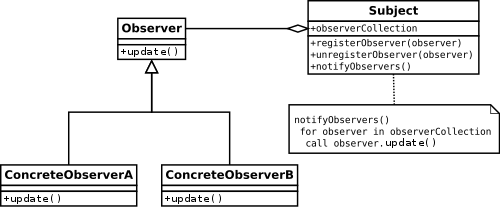
\includegraphics[width=\textwidth]{./assets/img/img019.png}
   \caption{Diagram UML wzorca ``Obserwator'' \cite{bib:url008}}
   \label{fig:19}
\end{figure}

\newpage

W projekcie został użyty także wzorzec ``Stan'' (Rysunek \ref{fig:20}). Pozwala on na ustawienie jakiegoś stanu aplikacji i odmiennych zachowań względem tego jak jest ustawiony. Przykładem w projekcie jest automatyczne podlewanie na płytce EcoDuino, które włączą i wyłącza daną funkcjonalność, w zależności od stanu zmiennej. Innym przykładem jest przycisk ``Start''/``Stop'' pompy w aplikacji desktop'owej, który w zależności od stanu, zmienia tekst i kolor.

\begin{figure}[H]
   \centering
   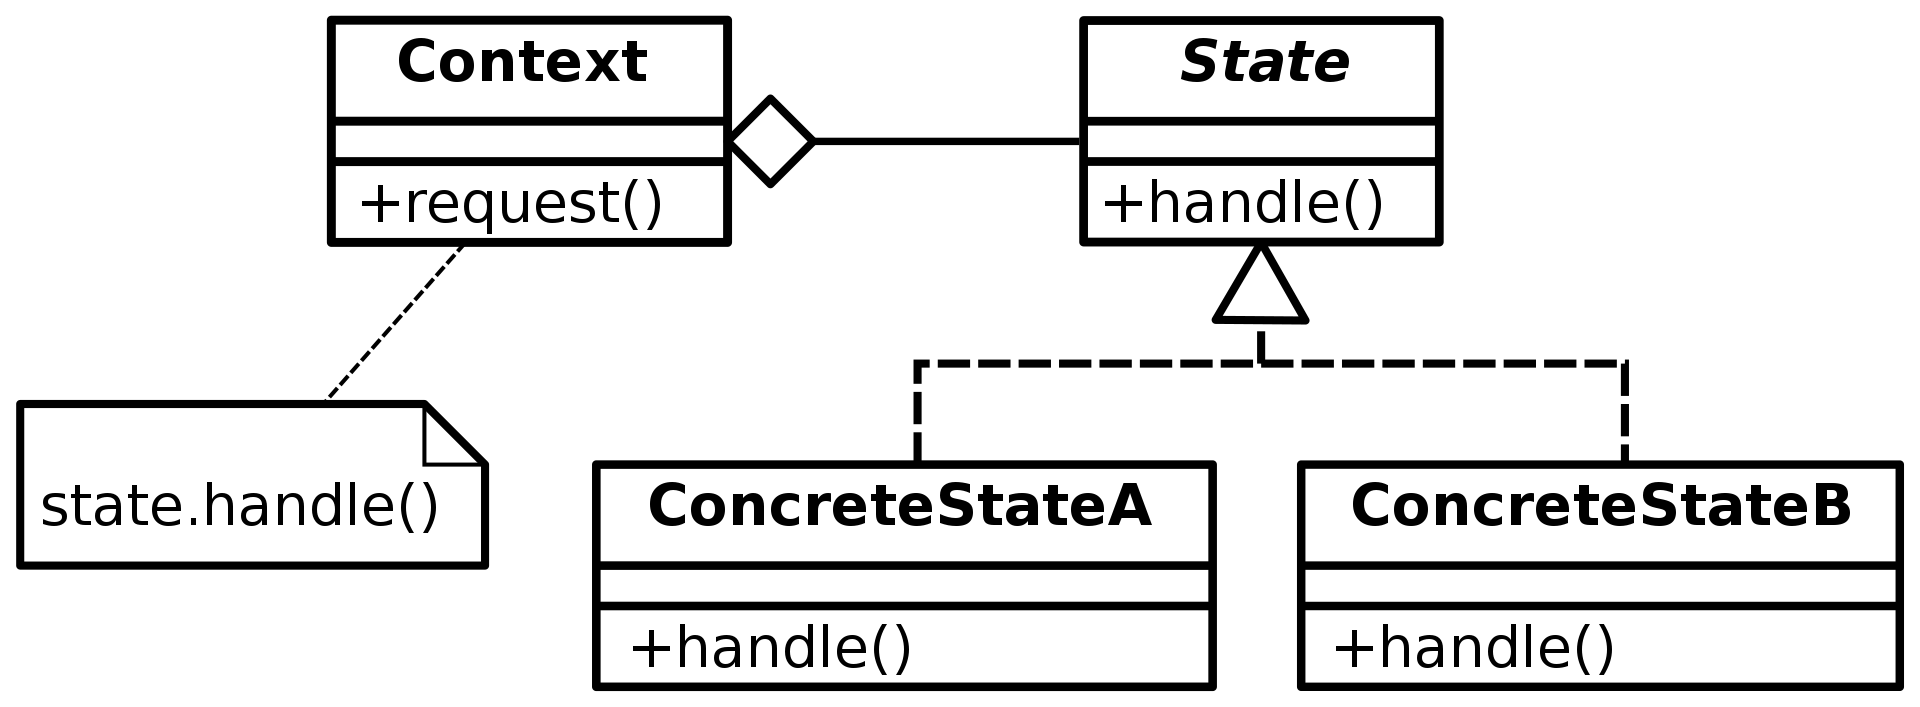
\includegraphics[width=\textwidth]{./assets/img/img020.png}
   \caption{Diagram klas UML programu na płytkę EcoDuino.}
   \label{fig:20}
\end{figure}

\newpage

\section{Diagramy UML}

Na rysunku \ref{fig:21} ukazany jest diagram klas programu na płytkę z zestawu EcoDuino.

\begin{figure}[H]
   \centering
   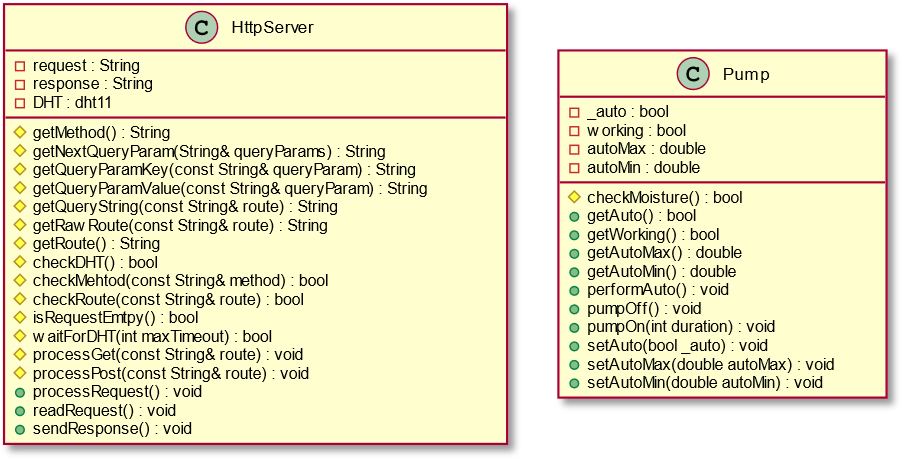
\includegraphics[width=\textwidth]{./assets/img/img021.png}
   \caption{Diagram UML wzorca ``Stan'' \cite{bib:url009}}
   \label{fig:21}
\end{figure}

Natomiast na rysunku \ref{fig:22} znajduje się diagram klas aplikacji desktop'owej.

\begin{figure}[H]
   \centering
   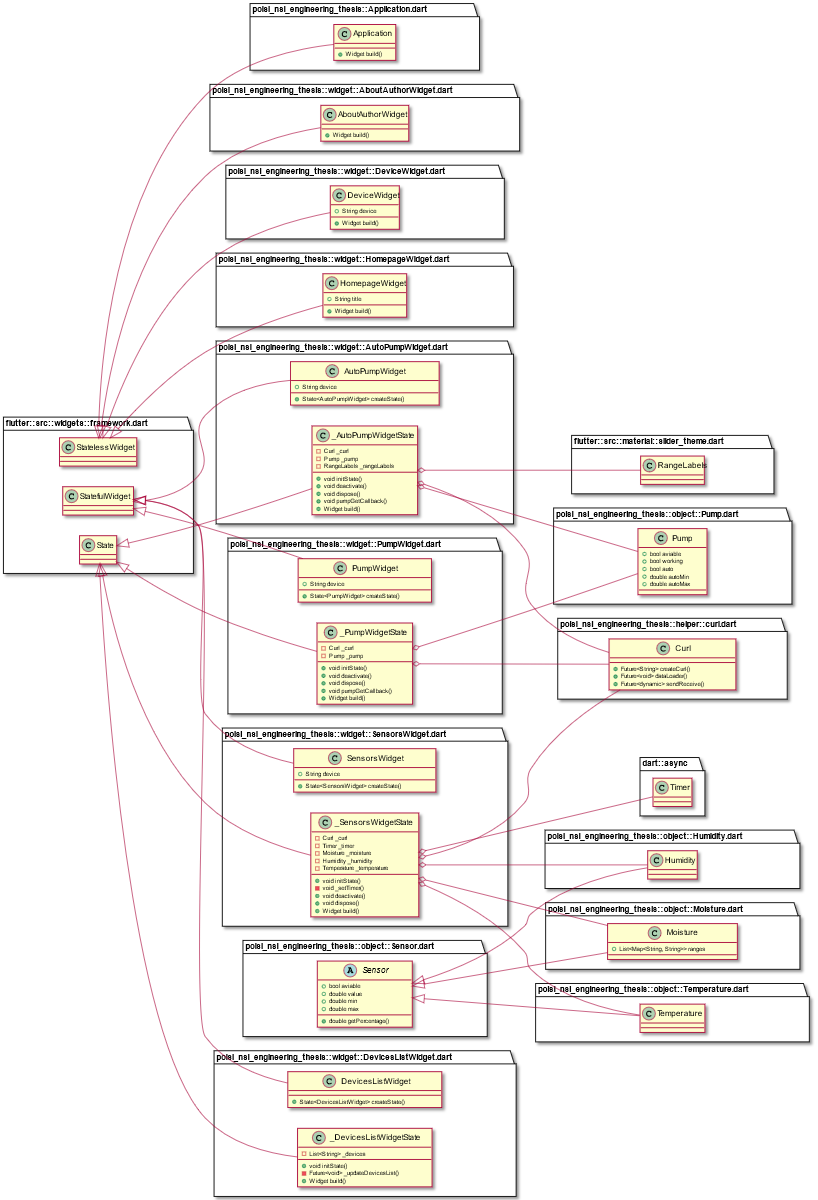
\includegraphics[width=\textwidth]{./assets/img/img022.png}
   \caption{Diagram klas UML aplikacji desktop'owej.}
   \label{fig:22}
\end{figure}

\chapter{Weryfikacja i walidacja}

W niniejszym rozdziale zostaną przedstawione sposoby weryfikacji i walidacji działania oprogramowania, przypadki testowe, zakres testowania, znalezione błędy oraz sposób ich wyeliminowania, a także wynik jednego z finalnych testów.

\section{Sposób testowania w ramach pracy}

Testowanie aplikacji przebiegało poszczególnymi etapami podczas procesu programowania.

Program na płytce z zestawu EcoDuino został przetestowany manualnie przy użyciu Serial Port Monitor'a.

W aplikacji desktop'owej do testowania zostały użyte testy manualne podczas kolejny części pisania aplikacji, ale także zostało napisanych kilka testów jednostkowych.

\section{Organizacja eksperymentów}

Do testowania programu na płytce z zestawu EcoDuino użyty został Serial Port Monitor, w którym wpisywane były poszczególne rządania i sprawdzane odpowiadające im zwrotki. Jeśli wszystko pasowało, dane z czujników były sczytane pomyślnie, albo pompa zostawała uruchamiana i zatrzymywana, test przechodził. W przeciwnym wypadku, gdy wystąpił błąd i coś nie działało, problem zostawał sprawdzany i naprawiany.

Podczas pisania aplikacji desktop'owej w Flutter'ze poszczególne części programu były testowane na bieżąco. Wykorzystywane w tym celu zostały testy manualne, które były najprostsze do wykonania oraz pozwalały na przegląd działania wszystkich funkcji w sytuacjach takich jakie może napotkać końcowy użytkownik. Oprócz testów manualnych zostały przygotowane testy jednostkowe sprawdzające poprawność wyświetlania kilku przykładowych widget'ów.

Testy manualne zostały przeprowadzone w dwóch środowiskach:

\begin{itemize}
   \item deweloperskim - podczas tworzenia oprogramowania, użyte do testów zostało pudełko z wodą, do której została włożona pompa, a czujniki zostały przetestowane odpowiednio nawilżając je wodą z pudełka, czy też dmuchając w przypadku czujnika wilgotności powietrza i temperatury,
   \item produkcyjnym - finalne testy przy użyciu prawdziwej rośliny i pudełka z wodą.
\end{itemize}

\section{Przypadki testowe, zakres testowania}

Najważniejszymi zakresami jakie zostały przetestowane były odpowiednio system wykonywania request'ów i response'ów na płytce EcoDuino, poszczególne rządania, działanie czujników, pompy i funkcji automatycznego podlewania, a także całości programu działającego na płytce.

Aplikacja została przetestowana pod kątem wyświetlania i działania każdego z dostępnych widget'ów. Dodatkową uwagę zwrócono na widget z danymi sczytywanymi z czujników urządzenia. Wszystkie rządania musiały zostać wykonywane asynchronicznie w taki sposób, aby użytkownik nie doświadczył zawieszenia aplikacji spowodowanych oczekiwaniem na odpowiedź z urządzenia.

Inną częścią aplikacji, która musiała zostać dokładniej przetestowana była funkcja automatycznego podlewania rośliny. Podczas powrotu do poprzedniego widget'u i ponownego wejścia na widget obsługujący automatyczne podlewanie, dane powinny zostać ponownie pobrane, a nie polegać na tych co były zapisane przy poprzednim wejściu.

\section{Wykryte i usunięte błędy}

Podczas testowania zostało wykrytych parę błędów, które zostały następnie naprawione. Zostaną one przedstawione poniżej.

Największym problemem jaki został wykryty był spadek wydajności aplikacji na widget'cie z czujnikami.

Na początku występował problem z strumieniem do odczytu danych z urządzenia, który był tworzony jako nowy obiekt przy każdym request'cie. Przez to, że obiekt ten nasłuchiwał na zmiany, nie zostawał on usunięty z pamięci, dlatego po kilku wywołaniach funkcji, zostało utworzonych zbyt duża ilość takich obiektów i osiągano limit dostępnych zasobów. Problem ten został naprawiony poprzez zamianę obiektu stream na funkcję sczytującą po 1 znaku, aż do napotkania znaku kończącego response.

Niestety nie naprawiło to w pełni problemu z wydajnością aplikacji na tym widget'cie. Każde rządania mimo tego, że zostało uruchomione asynchronicznie, wykonywało się w obrębie tego samego wątku, czego konsekwencją było wstrzymanie programu przy każdym odpytaniu. Rozwiązaniem było przeniesienie wywołań do osobnych, wyizolowanych wątków, dzięki czemu, problem z zatrzymywaniem się programu po wykonywaniu rządania został wyeliminowany.

Innym błędem jaki został zauważony podczas testów było ciągłe odpytywanie płytki o dane po wyjściu z widoku z czujnikami. Problem został zauważony podczas wyświetlania żądań i odpowiedzi używając polecenia ``print()''. Mimo tego, że został opuszczony widok z czujnikami, request'y nadal były wykonywane. Powodem takiego zachowania był ciągłe, nieprzerwane działanie funkcji ``periodic()'' klasy ``Timer''. Rozwiązaniem tego problemu było zakończenie działania Timer'a podczas opuszczania widget'u przy użyciu metody ``cancel()'' klasy ``Timer''.

\section{Opcjonalnie wyniki badań eksperymentalnych}

Jeden z finalnych testów został wykonany na prawdziwej roślinie Zamioculcas zamiolistnym (Rysunek \ref{fig:23}). Dane na temat wilgotności gleby jakie zostały sczytane to około 42\% (Rysunek \ref{fig:24}), co nie należało do najlepszych, ale też najgorszych wyników.

\begin{figure}[H]
   \centering
   \includegraphics[width=\textwidth,angle=270,origin=c]{./assets/img/img023.jpg}
   \caption{Test na prawdziwej roślinie.}
   \label{fig:23}
\end{figure}

\begin{figure}[H]
   \centering
   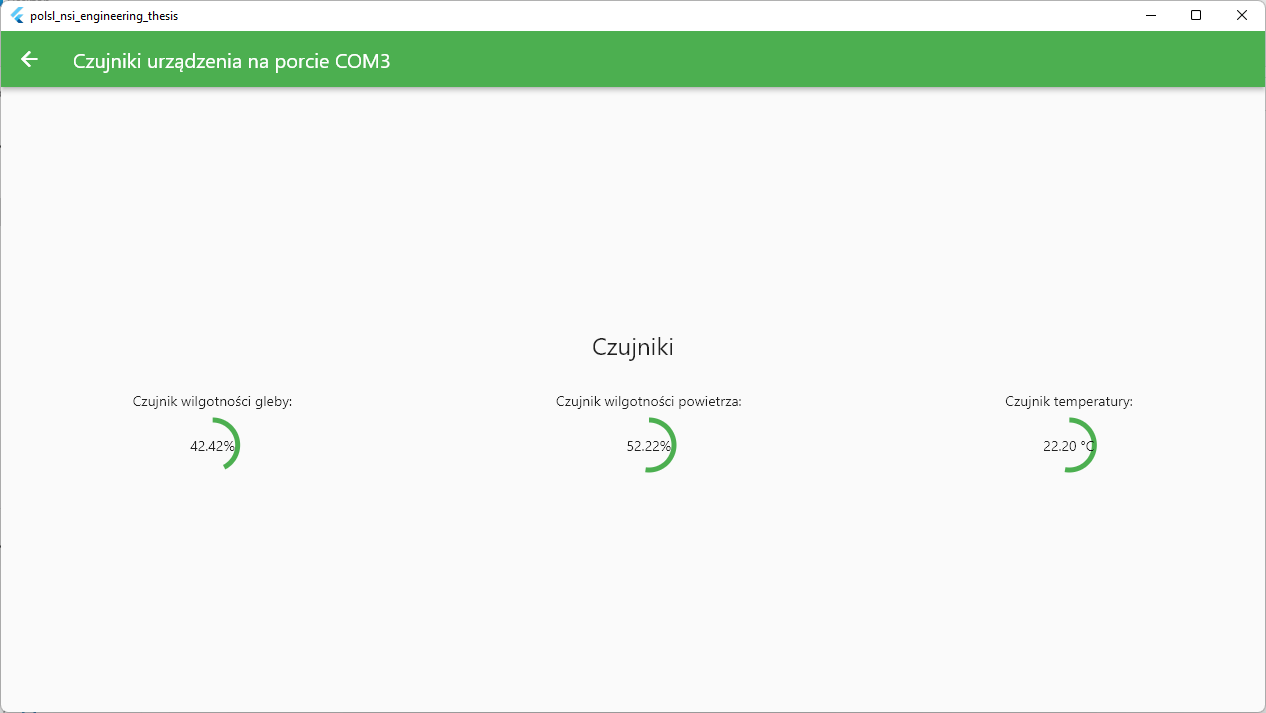
\includegraphics[width=\textwidth]{./assets/img/img024.png}
   \caption{Wyniki testu na prawdziwej roślinie.}
   \label{fig:24}
\end{figure}

\chapter{Podsumowanie i wnioski}

Projekt niniejszej pracy, który zakładał stworzenie systemu do monitorowania wilgotności gleby roślin doniczkowych, monitorowania temperatury i wilgotności otoczenia, nawadniania gleby oraz ustawienia automatycznego nawadniania w zależności od wilgotności gleby został zakończony z powodzeniem. Temat został odpowiednio przeanalizowany, zostały także wybrane właściwe do realizacji narzędzia i technologie, tak aby w finalnym efekcie został stworzony poprawnie działający system.

Podczas realizacji tworzenia systemu, zostało napotkanych kilka problemów, które zostały rozwiązane w czasie programowania. Największym problemem był wspomniany w podrozdziale 6.4 problem związany z wydajnością aplikacji desktop'owej na widget'cie z czujnikami, który powodował trudności, a nawet nie możliwość korzystania z aplikacji. Innym problemem, także opisanym w podrozdziałem 6.4 był niewidoczny dla użytkownika problem z brakiem zatrzymania Timer'a po wyjściu z widget'u z czujnikami, co powodowało niekończące się odpytywanie urządzenia o nowe dane, nawet jeśli nie było się na danym widget'cie.

Projekt ten posiada także potencjał na rozbudowę, poprzez użycie innych środków komunikacji takich jak Bluetooth lub WiFi oraz odpowiedniego ich zabezpieczenia. Rozbudowa ta pozwoliłaby końcowemu użytkownikowi na wygodniejszy sposób korzystania z urządzenia w niedużej odległości, bez konieczności podłączania się pod urządzenie.

Dana praca została wykonana w swoich założeniach i działa prawidłowo. Pozwoliła na wykonanie ciekawego projektu, który może zostać użyty, przez każdego człowieka potrzebującego systemu pomagającemu w opiece nad rośliną.

\bibliographystyle{plplain}
\bibliography{./assets/bib/bibliography}
\addcontentsline{toc}{chapter}{Bibliografia}


\begin{appendices}


   \chapter*{Spis skrótów i symboli}
   \addcontentsline{toc}{chapter}{Spis skrótów i symboli}

   \begin{itemize}
      \item[HTTP] Hypertext Transfer Protocol
      \item[REST] Representational state transfer
      \item[API] Application Programming Interface
      \item[JSON] JavaScript Object Notation
      \item[UX] User eXperience
      \item[FIFO] First In First Out
      \item[ASCII] American Standard Code for Information Interchange
   \end{itemize}


%    \chapter*{Źródła}
%    \addcontentsline{toc}{chapter}{Źródła}

%    Jeżeli w pracy konieczne jest umieszczenie długich fragmentów kodu źródłowego, należy je przenieść do załącznika.

%    \begin{lstlisting}
% partition fcm_possibilistic::doPartition
%                              (const dataset & ds)
% {
%    try
%    {
%       if (_nClusters < 1)
%          throw std::string ("unknown number of clusters");
%       if (_nIterations < 1 and _epsilon < 0)
%          throw std::string ("You should set a maximal number of iteration or minimal difference - epsilon.");
%       if (_nIterations > 0 and _epsilon > 0)
%          throw std::string ("Both number of iterations and minimal epsilon set -- you should set either number of iterations or minimal epsilon.");

%       auto mX = ds.getMatrix();
%       std::size_t nAttr = ds.getNumberOfAttributes();
%       std::size_t nX    = ds.getNumberOfData();
%       std::vector<std::vector<double>> mV;
%       mU = std::vector<std::vector<double>> (_nClusters);
%       for (auto & u : mU)
%          u = std::vector<double> (nX);
%       randomise(mU);
%       normaliseByColumns(mU);
%       calculateEtas(_nClusters, nX, ds);
%       if (_nIterations > 0)
%       {
%          for (int iter = 0; iter < _nIterations; iter++)
%          {
%             mV = calculateClusterCentres(mU, mX);
%             mU = modifyPartitionMatrix (mV, mX);
%          }
%       }
%       else if (_epsilon > 0)
%       {
%          double frob;
%          do
%          {
%             mV = calculateClusterCentres(mU, mX);
%             auto mUnew = modifyPartitionMatrix (mV, mX);

%             frob = Frobenius_norm_of_difference (mU, mUnew);
%             mU = mUnew;
%          } while (frob > _epsilon);
%       }
%       mV = calculateClusterCentres(mU, mX);
%       std::vector<std::vector<double>> mS = calculateClusterFuzzification(mU, mV, mX);

%       partition part;
%       for (int c = 0; c < _nClusters; c++)
%       {
%          cluster cl;
%          for (std::size_t a = 0; a < nAttr; a++)
%          {
%             descriptor_gaussian d (mV[c][a], mS[c][a]);
%             cl.addDescriptor(d);
%          }
%          part.addCluster(cl);
%       }
%       return part;
%    }
%    catch (my_exception & ex)
%    {
%       throw my_exception (__FILE__, __FUNCTION__, __LINE__, ex.what());
%    }
%    catch (std::exception & ex)
%    {
%       throw my_exceptionn (__FILE__, __FUNCTION__, __LINE__, ex.what());
%    }
%    catch (std::string & ex)
%    {
%       throw my_exception (__FILE__, __FUNCTION__, __LINE__, ex);
%    }
%    catch (...)
%    {
%       throw my_exception (__FILE__, __FUNCTION__, __LINE__, "unknown expection");
%    }
% }
% \end{lstlisting}


   \chapter*{Lista dodatkowych plików, uzupełniających tekst pracy}
   \addcontentsline{toc}{chapter}{Lista dodatkowych plików, uzupełniających tekst pracy}

   W systemie do pracy dołączono dodatkowe pliki zawierające:
   \begin{itemize}
      \item źródła programu,
      \item film pokazujący działanie opracowanego oprogramowania oraz zaprojektowanego i wykonanego urządzenia,
      \item prezentacja,
   \end{itemize}

   \listoffigures
   \addcontentsline{toc}{chapter}{Spis rysunków}
   % \listoftables
   % \addcontentsline{toc}{chapter}{Spis tabel}

\end{appendices}


\end{document}


%% Finis coronat opus.
